\chapter{有限元求解器画廊}
\label{ch:gallery}

\begin{quote}
本章的目标是展示一系列重要的内容
科学与工程学院的PDEs可以很快得到解决
FEniCS代码行。 我们从热方程开始,继续
用非线性Poisson方程,线性方程
弹性,Navier-Stokes方程式,最后看看如何
解决非线性对流 - 扩散反应的系统
方程。 这些问题说明了如何解决时间依赖性问题
问题,非线性问题,向量值问题和系统
PDEs。 对于每个问题,我们得出变分公式
在Python中以非常类似的方式表达问题
数学。
\end{quote}

\section{热方程式}
\label{ch:fundamentals:diffusion}

\index{heat equation}
\index{time-dependent problem}

作为前一章的Poisson问题的第一个扩展,
我们考虑时间依赖热方程,或时间依赖性
扩散方程。 这是Poisson的自然延伸
描述体内热量的固定分布的方程式
时间依赖的问题。

我们会看到,通过将时间离散成小时间间隔
采用标准时间步法,可以解决热量
通过求解一系列变分问题的方程式,很像
一个我们遇到的Poisson方程。

\subsection{PDE问题}

我们的时间依赖型PDE的模型问题读取

\begin{alignat}{2}
{\partial u\over\partial t} &= \nabla^2 u + f \quad &&\hbox{in }\Omega\times(0, T],
\label{ch:diffusion0:pde1}\\
u &= \ub &&\hbox{on } \partial \Omega\times(0, T],
\label{ch:diffusion0:pde1:bc}\\
u &= \uI &&\mbox{at } t=0\tp
\label{ch:diffusion0:pde1:ic}
\end{alignat}
在这里,$u$随空间和时间而变化,例如,如果空间,则$u=u(x,y,t)$
域$\Omega$是二维的。 源函数$f$和
边界值$\ub$也可能因空间和时间而异。
初始条件$\uI$仅是空间的函数。

\subsection{变化公式}
\label{ftut:timedep:diffusion1}

一个简单的方法来解决时间依赖的PDEs
有限元方法是首先离散时间导数a
有限差分近似,产生一个序列
固定问题,然后将每个静止问题转化为
变分公式

让上标$n$表示时间$t_n$的数量,其中$n$是一个
整数计数时间级别。 例如,$u^n$表示$u$在时间
级$n$。 时间上的有限差分离散化包括
在某个时间级别对PDE进行采样,说$t_{n + 1}$:

\index{time step}

\begin{equation}
\left({\partial u \over\partial t}\right)^{n+1} = \nabla^2 u^{n+1} + f^{n+1}\tp
\label{ch:diffusion0:pde1:tk}
\end{equation}
时间导数可以通过差商近似。
为了简单和稳定的原因,我们选择一个
简单向后的差异:

\index{implicit Euler}
\index{backward difference}

\begin{equation}
\left({\partial u\over\partial t}\right)^{n+1}\approx {{u^{n+1} - u^n}\over{\dt}},
\label{ch:diffusion0:BE}
\end{equation}
其中$\dt$是时间离散参数。
(\ref{ch:diffusion0:pde1:tk})插入(\ref{ch:diffusion0:BE})产生

\begin{equation}
{{u^{n+1} - u^n}\over{\dt}} = \nabla^2 u^{n+1} + f^{n+1}\tp
\label{ch:diffusion0:pde1:BE}
\end{equation}
这是我们的时间离散版本的热方程
(\ref{ch:diffusion0:pde1}),所谓的\emph{backward Euler}或\emph{implicit
  Euler}离散化。

我们可以重新排序(\ref{ch:diffusion0:pde1:BE})
左侧包含未知$u^{n+1}$的条款
右侧仅包含计算的条件。 结果
是假设为$u^{n+1}$的空间(静态)问题的序列
$u^n$从以前的时间步长是已知的:

\begin{align}
u^0 &= \uI, \label{ch:diffusion0:pde1:u0}\\
u^{n+1} - {\dt}\nabla^2 u^{n+1} &=  u^n + {\dt} f^{n+1},\quad n=0,1,2,\ldots
\label{ch:diffusion0:pde1:uk}
\end{align}

给定$\uI$,我们可以解决$u^0$,$u^1$,$u^2$等。

(\ref{ch:diffusion0:pde1:uk})的替代方法,可以是
方便实施,是收集
平等标志一方的所有术语:

\begin{equation}
u^{n+1} - {\dt}\nabla^2 u^{n+1} -  u^{n} - {\dt} f^{n+1} = 0,\quad n=0,1,2,\ldots
\label{ch:diffusion0:pde1:uk2}
\end{equation}

我们使用有限元方法来解决
(\ref{ch:diffusion0:pde1:u0})和任一方程式
(\ref{ch:diffusion0:pde1:uk})或(\ref{ch:diffusion0:pde1:uk2})。 这个
需要将方程式变为弱形式。 像往常一样,我们倍增
通过一个测试函数$v\in \hat V$并将二阶导数合并
部分。 在$u^{n+1}$(这是自然的)中引入符号$u$
程序),由此产生的弱势形式
配方(\ref{ch:diffusion0:pde1:uk})
可以方便地写入
标准符号:

\[ a(u,v)=L_{n+1}(v),\]
哪里

\begin{align}
a(u,v) &= \int_\Omega\left(uv + {\dt}
\nabla u\cdot \nabla v\right) \dx, \label{ch:diffusion0:pde1:a}\\
L_{n+1}(v) &= \int_\Omega \left(u^n + {\dt}  f^{n+1}\right)v \dx\tp
\label{ch:diffusion0:pde1:L}
\end{align}
替代形式(\ref{ch:diffusion0:pde1:uk2})有一个
抽象配方

\[ F_{n+1}(u;v) = 0,\]
哪里

\begin{equation}
F_{n+1}(u; v) = \int_\Omega \left(uv + {\dt}
\nabla u\cdot \nabla v -
(u^n + {\dt} f^{n+1})v\right) \dx\tp
\label{ch:diffusion0:pde1:F}
\end{equation}

除了每个时间步长要解决的变化问题外,
我们还需要近似初始条件
(\ref{ch:diffusion0:pde1:u0})。 这个方程也可以变成a
变分问题:

\[ a_0(u,v)=L_0(v),\]
哪里

\begin{align}
a_0(u,v) &= \int_\Omega uv \dx, \label{ch:diffusion0:pde1:a0}\\
L_0(v) &= \int_\Omega \uI v \dx\tp \label{ch:diffusion0:pde1:L0}
\end{align}
当解决这个变分问题时,$u^0$成为$L^2$
将给定的初始值$\uI$投影到有限元中
空间。 另一种方式是通过内插来构造$u^0$
初始值$\uI$; 也就是说,如果$u^0=\sum_{j=1}^N U^0_j\phi_j$,我们
只需设置$U_j=\uI(x_j,y_j)$,其中$(x_j,y_j)$是坐标
节点编号$j$。 我们将这两个策略称为计算
初始条件通过投影或插值。 都
在FEniCS中通过单一语句轻松计算操作,
使用\texttt{project}或\texttt{interpolate}函数。 最常见的
选择是\texttt{project},它计算一个近似值为$\uI$,但是在
一些我们想通过再现来验证代码的应用程序
确切的解决方案,必须使用\texttt{interpolate}(我们使用这样的测试
这里的问题!)。

\index{interpolate@{\rm\texttt{interpolate}}}
\index{project@{\rm\texttt{project}}}

总之,我们需要解决以下变分序列
计算热方程有限元解的问题:
找到$u^0\in V$,以便$a_0(u^0,v)=L_0(v)$对于所有$v\in\hat V$,
然后找到$u^{n+1}\in V$
使得$a(u^{n+1},v)=L_{n+1}(v)$对于$v\in\hat V$,
或者,对于$v\in\hat V$中的$F_{n+1}(u^{n+1},v)=0$,
$n=0,1,2,\ldots$。

\subsection{FEniCS实现}
\label{ftut:timedep:diffusion1:impl}

我们的程序需要手动实现时间步伐,但可以
依靠FEniCS轻松计算$a_0$,$L_0$,$a$和$L$(或
$F_{n+1}$),并解决未知数的线性系统。

\paragraph{测试问题1:一个已知的分析解决方案。}
就像前一章的Poisson问题一样,我们
构建一个测试问题,使其容易确定是否
计算正确。 既然我们知道我们的一流
时间步长方案对于线性函数是精确的,我们创建一个测试
时间线性变化的问题。 我们把这与一个
空间二次变化。 我们因此而来

\begin{equation} u = 1 + x^2 + \alpha y^2 + \beta t,
\label{ch:diffusion0:pde1:u0test}
\end{equation}
其产生了在节点处的计算值将是的函数
确切的,不管元素的大小和$\dt$,只要
网格被均匀分割。 插入
(\ref{ch:diffusion0:pde1:u0test})转换为热方程
(\ref{ch:diffusion0:pde1}),我们发现右边的$f$必须
由$f(x,y,t)=\beta - 2 - 2\alpha$给出。 边界值
是$\ub(x,y,t)= 1 + x^2 + \alpha y^2 + \beta t$和初始
值为$\uI(x,y)= 1 + x^2 + \alpha y^2$。

\paragraph{FEniCS实现。}
一个新的编程问题是如何处理不同的功能
空间和时间,如边界条件$\ub(x,y,
t)= 1 + x^2 + \alpha y^2 + \beta t$。 一个自然的解决方案是使用
FEniCS \texttt{Expression}与time $t$作为参数,除了
参数$\alpha$和$\beta$:

\index{time-dependent expression}

\begin{python}
alpha = 3; beta = 1.2
u_D = Expression('1 + x[0]*x[0] + alpha*x[1]*x[1] + beta*t',
                 degree=2, alpha=alpha, beta=beta, t=0)
\end{python}
\texttt{Expression}将\texttt{x}的组件用作独立的
变量,而\texttt{alpha},\texttt{beta}和\texttt{t}是参数。该
time \texttt{t}可以稍后更新

\begin{python}
u_D.t = t
\end{python}

在这种情况下,沿着整个边界的基本边界条件,
以与我们以前实施的相同的方式实施
泊松问题的边界条件:

\begin{python}
def boundary(x, on_boundary):
    return on_boundary

bc = DirichletBC(V, u_D, boundary)
\end{python}

我们将使用变量\texttt{u}作为新的未知$u^{n+1}$
时间步长和变量\verb!u_n! 对于上一次的$u^n$
步。 \verb!u_n!的初始值可以通过任一投影来计算
或插值$\uI$。 由于我们为边界值设置了\texttt{t = 0}
\verb!u_D!,我们可以使用\verb!u_D! 指定初始条件:

\begin{python}
u_n = project(u_D, V)
# or
u_n = interpolate(u_D, V)
\end{python}

\begin{notice}[投影与内插初始条件]
实际恢复确切的解决方案
(\ref{ch:diffusion0:pde1:u0test})到机器精度,这很重要
通过内插$\uI$来计算离散的初始条件。 这个
确保自由度是准确的(机器精度)
在$t=0$。 投影导致节点处的近似值。
\end{notice}

\index{lhs@{\rm\texttt{lhs}}}
\index{rhs@{\rm\texttt{rhs}}}
\index{projection}
\index{interpolation}

我们可以根据上述公式定义$a$或$L$,或者我们
可能只是定义$F$,并要求FEniCS找出哪些术语应该去
进入双线性形式$a$,并且应该进入线性形式
$L$。 后者是方便的,特别是在更复杂的
问题,所以我们说明了建设$a$和$L$:

\begin{python}
u = TrialFunction(V)
v = TestFunction(V)
f = Constant(beta - 2 - 2*alpha)

F = u*v*dx + dt*dot(grad(u), grad(v))*dx - (u_n + dt*f)*v*dx
a, L = lhs(F), rhs(F)
\end{python}

最后,我们在循环中执行时间步长:

\begin{python}
u = Function(V)
t = 0
for n in range(num_steps):

    # Update current time
    t += dt
    u_D.t = t

    # Solve variational problem
    solve(a == L, u, bc)

    # Update previous solution
    u_n.assign(u)
\end{python}
在时间步长循环的最后一步,我们分配值
变量\texttt{u}(新计算的解决方案)变量\verb!u_n!
包含上一个时间步长的值。 必须这样做
使用\texttt{assign}成员函数。 如果我们反而尝试做\verb!u_n = u!,
我们将设置\verb!u_n! 变量与\texttt{u}变量相同
这不是我们想要的。 (我们需要两个变量,一个是值
在前一个时间步长,另一个是当前时间的值
步。)

\begin{notice}[记住用当前时间更新表达式对象!]
在时间循环内,观察\verb!u_D.t! 必须在之前更新
\texttt{solve}语句强制执行Dirichlet条件的计算
当前时间步长。 一个Dirichlet条件定义为a
\texttt{Expression}查找并应用参数的值,如\texttt{t}
当它被评估并应用于线性系统时。
\end{notice}

上面的时间步进循环不包含任何比较
数字和确切的解决方案,我们必须包括为了
验证实施。 至于Poisson方程式
部分~\ref{ch:poisson0:impl:dissect},我们计算差异
在\texttt{u}的节点数组和节点数组之间
内插精确解的值。 这可以做到
如下:

\begin{python}
u_e = interpolate(u_D, V)
error = np.abs(u_e.vector().array() - u.vector().array()).max()
print('t = %.2f: error = %.3g' % (t, error))
\end{python}
对于Poisson示例,我们使用了这个函数
\verb!compute_vertex_values! 提取功能值
顶点。 这里我们举例说明一种提取方法
顶点值,通过调用函数\texttt{vector}返回
自由度向量。 对于$\mathsf{P}_1$
功能空间,这个矢量的自由度将等于
通过调用获得的顶点值数组
\verb!compute_vertex_values!,虽然可能有不同的顺序。

解决热方程的完整程序如下:

\begin{python}
from fenics import *
import numpy as np

T = 2.0            # final time
num_steps = 10     # number of time steps
dt = T / num_steps # time step size
alpha = 3          # parameter alpha
beta = 1.2         # parameter beta

# Create mesh and define function space
nx = ny = 8
mesh = UnitSquareMesh(nx, ny)
V = FunctionSpace(mesh, 'P', 1)

# Define boundary condition
u_D = Expression('1 + x[0]*x[0] + alpha*x[1]*x[1] + beta*t',
                 degree=2, alpha=alpha, beta=beta, t=0)

def boundary(x, on_boundary):
    return on_boundary

bc = DirichletBC(V, u_D, boundary)

# Define initial value
u_n = interpolate(u_D, V)
#u_n = project(u_D, V)

# Define variational problem
u = TrialFunction(V)
v = TestFunction(V)
f = Constant(beta - 2 - 2*alpha)

F = u*v*dx + dt*dot(grad(u), grad(v))*dx - (u_n + dt*f)*v*dx
a, L = lhs(F), rhs(F)

# Time-stepping
u = Function(V)
t = 0
for n in range(num_steps):

    # Update current time
    t += dt
    u_D.t = t

    # Compute solution
    solve(a == L, u, bc)

    # Plot solution
    plot(u)

    # Compute error at vertices
    u_e = interpolate(u_D, V)
    error = np.abs(u_e.vector().array() - u.vector().array()).max()
    print('t = %.2f: error = %.3g' % (t, error))

    # Update previous solution
    u_n.assign(u)

# Hold plot
interactive()
\end{python}
该示例程序可以在文件中找到
\begin{center}
  \url{https://fenicsproject.org/pub/tutorial/python/vol1/ft03_heat.py}
\end{center}
\begin{center}
  {\nolinkurl{ft03_heat.py}}
\end{center}

\index{ft03\_heat.py@{\rm\texttt{ft03\_heat.py}}}

\paragraph{测试问题2:Gaussian函数的扩散。}
让我们现在解决一个更有趣的测试问题,即扩散
一个Gaussian山。 我们以初始值为准

\[ \uI(x,y)= e^{-ax^2 - ay^2}\]
在$a = 5$的域$[-2,2]\times [2,2]$。 为了这
问题我们将使用均匀的Dirichlet边界条件($\ub = 0$)。

\paragraph{FEniCS实现。}
以前的程序需要修改哪些? 一个专业
更改是域不再是单位平方。 新域名可以
使用\texttt{RectangleMesh}在FEniCS中轻松创建:

\begin{python}
nx = ny = 30
mesh = RectangleMesh(Point(-2, -2), Point(2, 2), nx, ny)
\end{python}
请注意,我们比以前使用了比以前更高的分辨率
解决解决方案的功能。 我们还需要重新定义
初始条件和边界条件。 两者都很容易改变
定义一个新的\texttt{Expression},并在边界上设置$u = 0$。

能够在外部程序中可视化解决方案,如
ParaView,我们将每次将解决方案保存为VTK格式的文件
步。 我们首先用后缀\texttt{.pvd}创建一个\texttt{File}:

\begin{python}
vtkfile = File('heat_gaussian/solution.pvd')
\end{python}
在时间循环中,我们可能会将解值附加到
这个文件:

\begin{python}
vtkfile << (u, t)
\end{python}
在每个时间步骤中调用此行,从而创建
一个包含后缀\texttt{.vtu}的新文件,其中包含时间步长的所有数据
(网格和顶点值)。 文件
\verb!heat_gaussian/solution.pvd! 将包含时间值和
引用\texttt{.vtu}文件,这意味着\texttt{.pvd}文件将是
单个小文件指向大量\texttt{.vtu}文件
包含实际数据。 请注意,我们选择存储解决方案
到一个名为\verb!heat_gaussian!的子目录。 这是为了避免混乱
我们的源目录与所有生成的数据文件。
在运行之前不需要创建目录
程序将由FEniCS自动创建。

\index{VTK format}
\index{.pvd@{\rm\texttt{.pvd}} file}
\index{.vtu@{\rm\texttt{.vtu}} file}

完整的程序如下所示。

\begin{python}
from fenics import *
import time

T = 2.0            # final time
num_steps = 50     # number of time steps
dt = T / num_steps # time step size

# Create mesh and define function space
nx = ny = 30
mesh = RectangleMesh(Point(-2, -2), Point(2, 2), nx, ny)
V = FunctionSpace(mesh, 'P', 1)

# Define boundary condition
def boundary(x, on_boundary):
    return on_boundary

bc = DirichletBC(V, Constant(0), boundary)

# Define initial value
u_0 = Expression('exp(-a*pow(x[0], 2) - a*pow(x[1], 2))',
                 degree=2, a=5)
u_n = interpolate(u_0, V)

# Define variational problem
u = TrialFunction(V)
v = TestFunction(V)
f = Constant(0)

F = u*v*dx + dt*dot(grad(u), grad(v))*dx - (u_n + dt*f)*v*dx
a, L = lhs(F), rhs(F)

# Create VTK file for saving solution
vtkfile = File('heat_gaussian/solution.pvd')

# Time-stepping
u = Function(V)
t = 0
for n in range(num_steps):

    # Update current time
    t += dt

    # Compute solution
    solve(a == L, u, bc)

    # Save to file and plot solution
    vtkfile << (u, t)
    plot(u)

    # Update previous solution
    u_n.assign(u)

# Hold plot
interactive()
\end{python}
该示例程序可以在文件中找到
\begin{center}
  \url{https://fenicsproject.org/pub/tutorial/python/vol1/ft04_heat_gaussian.py}
\end{center}
\begin{center}
  {\nolinkurl{ft04_heat_gaussian.py}}
\end{center}

\index{ft04\_heat\_gaussian.py@{\rm\texttt{ft04\_heat\_gaussian.py}}}

\paragraph{ParaView中的可视化。}
为了可视化高斯山的扩散,启动ParaView,
选择\textbf{File--Open...},打开
\verb!heat_gaussian/solution.pvd!,然后点击
\textbf{Apply}在Properties窗格中。 点击播放按钮进行显示
解决方案的动画。 要将动画保存到文件中,请单击
\textbf{File--Save Animation...}并将文件保存为所需的文件格式,
例如AVI或Ogg/Theora。
动画一旦保存到文件中,就可以播放动画
离线使用播放器,如mplayer或VLC,或上传您的
动画到YouTube。 图~\ref{fig:snapshots}显示了一个序列
的解决方案的快照。

%\begin{figure}[!ht]  % fig:snapshots
%  \centerline{
\includegraphics[width=0.95\linewidth]{fig/heat.png}}
%  \caption{
%  A sequence of snapshots of the solution of the Gaussian hill problem created with ParaView. \label{fig:snapshots}
%  }
%\end{figure}

\section{非线性Poisson方程}
\label{ftut1:gallery:nonlinearpoisson}

\index{nonlinear problem}

现在我们将介绍如何解决非线性PDE问题。 我们会看到
非线性问题可以像线性问题那样容易地解决
FEniCS,通过简单地定义非线性变分问题和调用
\texttt{solve}功能。 当这样做时,我们会遇到一个微妙的
变分问题如何定义的差异。

\subsection{PDE问题}

作为解决非线性PDE的模型问题,我们
取以下非线性Poisson方程:

\begin{equation}
-\nabla\cdot\left(q(u)\nabla u\right) = f,
\end{equation}
在$\Omega$中,$u=\ub$在边界$\partial\Omega$上。
系数$q = q(u)$使得方程非线性(除非$q(u)$
在$u$中是不变的)。

\subsection{变化公式}

像往常一样,我们的PDE乘以一个测试函数$v\in\hat V$,
整合域,并整合二阶导数
按部件。 由零件整合产生的边界积分
无论我们使用Dirichlet条件,都会消失。 所结果的
我们的模型问题的变分公式变成:找到$u \in V$
就这样

\begin{equation}
F(u; v) = 0 \quad \forall v \in \hat{V},
\label{ch:poisson0:nonlinear1}
\end{equation}
哪里

\begin{equation}
F(u; v) = \int_\Omega (q(u)\nabla u\cdot \nabla v - fv) \dx,
\label{ch:poisson0:nonlinear2}
\end{equation}
和

\begin{align*}
     V      &= \{v \in H^1(\Omega) : v = \ub \mbox{ on } \partial\Omega\},\\
    \hat{V} &= \{v \in H^1(\Omega) : v = 0 \mbox{ on } \partial\Omega\}\tp
\end{align*}

离散的问题像往常一样通过限制$V$和$\hat V$出现
到一对离散空间。 像以前一样,我们省略了任何下标
离散空间和离散解。
然后将离散的非线性问题写为:找到$u \in V$

\begin{equation}
  F(u; v) = 0 \quad \forall v \in \hat{V},
\label{ch:poisson0:nonlinear:d}
\end{equation}
与$u = \sum_{j=1}^N U_j \phi_j$。 由于$F$是非线性的
$u$,变量语句产生一个系统
未知数$U_1,\ldots,U_N$中的非线性代数方程。

\subsection{FEniCS实现}
\label{ftut:nonlinear:Newton:auto}

\paragraph{测试问题。}
为了解决测试问题,我们需要选择右边的$f$,
系数$q(u)$和边界值$\ub$。 以前,我们
与制造的解决方案一起工作,可以无需复制
近似误差 这在非线性问题上更为困难,
代数更加繁琐。 但是,我们可以利用SymPy
符号计算,并将这些计算集成到FEniCS中
求解。 这允许我们轻松地尝试不同的
制造解决方案。 SymPy的即将到来的代码需要一些
基本熟悉这个包。 特别是我们会用
SymPy函数\texttt{diff}用于符号区分和\texttt{ccode} for
C/C++代码生成。

我们取$q(u) = 1 + u^2$并定义二维制造
$x$和$y$中的线性解决方案:

\begin{python}
# Warning: from fenics import * will import both `sym` and
# `q` from FEniCS. We therefore import FEniCS first and then
# overwrite these objects.
from fenics import *

def q(u):
    "Return nonlinear coefficient"
    return 1 + u**2

# Use SymPy to compute f from the manufactured solution u
import sympy as sym
x, y = sym.symbols('x[0], x[1]')
u = 1 + x + 2*y
f = - sym.diff(q(u)*sym.diff(u, x), x) - sym.diff(q(u)*sym.diff(u, y), y)
f = sym.simplify(f)
u_code = sym.printing.ccode(u)
f_code = sym.printing.ccode(f)
print('u =', u_code)
print('f =', f_code)
\end{python}

\index{SymPy}
\index{method of manufactured solutions}

\begin{notice}[在\texttt{Expression}对象中根据需要定义符号坐标]
请注意,我们通常会写\texttt{x,y = sym.symbols('x,y')},但是
如果我们希望生成的表达式具有有效的语法
FEniCS \texttt{Expression}对象,我们必须使用\texttt{x[0]}和\texttt{x[1]}。
通过定义\texttt{x}的名称,\texttt{sympy}可以轻松实现这一点
\texttt{y} as \texttt{x[0]}和\texttt{x[1]}:\texttt{x,y = sym.symbols('x[0], x[1]')}。
\end{notice}

将\texttt{u}和\texttt{f}的表达式转换为C或C ++语法
FEniCS \texttt{Expression}对象需要两个步骤。 首先,我们要求C
表达式的代码:

\begin{python}
u_code = sym.printing.ccode(u)
f_code = sym.printing.ccode(f)
\end{python}
在某些情况下,需要编辑结果以匹配所需的结果
\texttt{Expression}对象的语法,但不是这种情况。 (首要的
例如\verb!M_PI! 对于$\pi$在C/C++中必须由\texttt{pi}替代
\texttt{Expression}对象。)在本例中,\verb!u_code!的输出 和
\verb!f_code!是

\begin{c}
x[0] + 2*x[1] + 1
-10*x[0] - 20*x[1] - 10
\end{c}
定义网格,功能空间和边界后,
我们定义边界值\verb!u_D! 如

\begin{python}
u_D = Expression(u_code, degree=1)
\end{python}
类似地,我们定义右边的函数

\begin{python}
f = Expression(f_code, degree=1)
\end{python}

\begin{notice}[命名FEniCS与程序变量之间的冲突]
在上面的程序中,可能会出现奇怪的错误
名字冲突。 如果在做之前定义\texttt{sym}和\texttt{q}
\texttt{from fenics import *},后一个语句也会导入
变量名为\texttt{sym}和\texttt{q},覆盖
你以前定义的对象! 这可能会导致奇怪
错误。 最安全的解决方案是做\texttt{import fenics}而不是
\texttt{from fenics import *},然后前缀所有FEniCS
\texttt{fenics}的对象名称。 下一个最好的解决办法就是做
\texttt{from fenics import *}首先定义你自己的变量
覆盖从\texttt{fenics}导入的那些。 这是可以接受的
如果我们不需要\texttt{fenics}中的\texttt{sym}和\texttt{q}。
\end{notice}

\paragraph{FEniCS实现。}
非线性Poisson方程的求解器很容易
实现线性Poisson方程的求解器。
我们所需要做的就是说明$F$和调用的公式
\texttt{solve(F == 0,u,bc)},而不是\texttt{solve(a == L,u,bc)}
在线性情况下。 这是一个简约代码:

\begin{python}
from fenics import *

def q(u):
    return 1 + u**2

mesh = UnitSquareMesh(8, 8)
V = FunctionSpace(mesh, 'P', 1)
u_D = Expression(u_code, degree=1)

def boundary(x, on_boundary):
    return on_boundary

bc = DirichletBC(V, u_D, boundary)

u = Function(V)
v = TestFunction(V)
f = Expression(f_code, degree=1)
F = q(u)*dot(grad(u), grad(v))*dx - f*v*dx

solve(F == 0, u, bc)
\end{python}

该示例程序的完整版本可以在该文件中找到
\begin{center}
\url{https://fenicsproject.org/pub/tutorial/python/vol1/ft05_poisson_nonlinear.py}
\end{center}
\begin{center}
{\nolinkurl{ft05_poisson_nonlinear.py}}
\end{center}

\index{ft05\_poisson\_nonlinear.py@{\rm\texttt{ft05\_poisson\_nonlinear.py}}}

与线性问题的主要区别在于未知功能
\texttt{u}在非线性情况下的变分形式
必须定义为\texttt{Function},而不是\texttt{TrialFunction}。 在某种意义上
这是从线性情况的简化,我们必须定义\texttt{u}
首先作为\texttt{TrialFunction}然后作为\texttt{Function}。

\index{Newton's method}
\index{Jacobian}

\texttt{solve}函数采用非线性方程,从符号出发
Jacobian矩阵,并运行一个Newton方法来计算解。

当我们运行代码时,FEniCS会报告Newton的进度
迭代。 以$2\cdot(8\times 8)$单元格,我们达到8的收敛
具有容忍度$10^{-9}$的迭代,以及错误
数值解约为$10^{-16}$。 这些结果带来了证据
为正确的实施。 思考有限差异
在均匀网格上,$\mathsf{P}_1$元素模拟标准
二阶差分,其计算线性的导数或
二次函数。 在这里,$\nabla u$是一个常量向量,但是
然后乘以$(1+u^2)$,它是二阶多项式
$x$和$y$,分歧“差异运算符”应该是
准确计算。 因此,我们可以使用$\mathcal{P}_1$
元素,期望制造的$u$被转载
数值方法。 像$1+u^4$这样的非线性,这不会是
情况,我们需要验证收敛率。

目前的例子显示了解决非线性问题的难易程度
在FEniCS。 但是,专家对非线性的数值解
PDEs非常了解,非线性的自动化程序可能会失败
问题,通常需要有更好的手册
解决方案的流程控制比我们目前的流程要好
案件。 我们在\cite{ftut2}中返回此问题,并显示如何
实现非线性方程式的定制解算法
我们如何引导使用的自动化Newton方法中的参数
以上。

\section{线性弹性方程}
\label{ftut:elast}

\index{elasticity}
\index{system of PDEs}

结构分析是现代主要活动之一
工程,这可能使PDE建模变形
弹性体是世界上最流行的PDE。 只需一个
用于解决FEniCS中2D或3D弹性方程的代码页,
具体细节如下。

\subsection{PDE问题}

\index{stress tensor}
\index{tensor}

控制身体的小弹性变形的方程式$\Omega$的方程式
可以写成

\begin{align}
-\nabla\cdot\sigma &= f\hbox{ in }\Omega,
\label{ftut:elast:varform:equilibrium}\\
\sigma &= \lambda\,\hbox{tr}\,(\varepsilon) I + 2\mu\varepsilon,
\label{ftut:elast:varform:stresstrain}\\
\varepsilon &= \frac{1}{2}\left(\nabla u + (\nabla u)^{\top}\right),
\label{ftut:elast:varform:strainu}
\end{align}
其中$\sigma$是压力张量,$f$是每单位的身体力量
卷,$\lambda$和$\mu$是$\text{Lam\'e's}$弹性参数为
物品在$\Omega$,$I$是身份张量,$\mathrm{tr}$是
跟踪运算符在张量上,$\varepsilon$是对称应变率
张量(对称梯度),$u$是位移矢量场。
我们这里假设各向同性弹性条件。

我们结合在一起 (\ref{ftut:elast:varform:stresstrain}) 和
(\ref{ftut:elast:varform:strainu}) 获得

\begin{equation}
\sigma = \lambda(\nabla\cdot u)I + \mu(\nabla u + (\nabla u)^{\top})\tp
\label{ftut:elast:varform:stressu}
\end{equation}
注意
(\ref{ftut:elast:varform:equilibrium})--(\ref{ftut:elast:varform:strainu})
可以轻松地转换为$u$的单个向量PDE,这是
管理未知$u$(Navier方程)的PDE。 在里面
然而,变分式的推导是方便的
保持方程式如上所述。

\subsection{变化公式}
\label{ftut:elast:varform}

变分公式
(\ref{ftut:elast:varform:equilibrium})--(\ref{ftut:elast:varform:strainu})
包括形成内部产品
(\ref{ftut:elast:varform:equilibrium})和一个\emph{vector}测试函数
$v\in \hat{V}$,其中$\hat{V}$是向量值的测试函数空间,
整合域$\Omega$:

\[ -\int_\Omega (\nabla\cdot\sigma) \cdot v \dx =
\int_\Omega f\cdot v\dx\tp\]
由于$\nabla\cdot\sigma $包含主要的二阶导数
未知$u$,我们将这个术语整合在一起:

\[ -\int_\Omega (\nabla\cdot\sigma) \cdot v \dx
= \int_\Omega \sigma : \nabla v\dx - \int_{\partial\Omega}
(\sigma\cdot n)\cdot v \ds,\]
冒号运算符是张量之间的内积(相加
所有元素的成对产品),$n$是向外单位正常
在边界。 数量$\sigma\cdot n$被称为
牵引力或应力矢量在边界,并经常规定
作为边界条件。 我们在这里假定它是在部分规定的
$\partial\Omega_T$的边界为$\sigma\cdot n = T$。 在上
剩下的一部分边界,我们假设的价值
位移作为Dirichlet条件给出。 我们得到了

\[
\int_\Omega \sigma : \nabla v \dx =
\int_\Omega f\cdot v \dx
+ \int_{\partial\Omega_T} T\cdot v\ds\tp\]
插入表达式(\ref{ftut:elast:varform:stressu})
$\sigma$给出$u$的变体形式为未知。 请注意
剩余部分的边界积分
由于Dirichlet,$\partial\Omega\setminus\partial\Omega_T$消失
条件。

我们现在可以将变分公式总结为:找到$u\in V$

\begin{equation}
a(u,v) = L(v)\quad\forall v\in\hat{V},
\end{equation}
哪里

\begin{align}
a(u,v) &= \int_\Omega\sigma(u) :\nabla v \dx,
\label{ftut:elast:varform:sigma_inner_gradv}
\\
\sigma(u) &= \lambda(\nabla\cdot u)I + \mu(\nabla u + (\nabla u)^{\top}),\\
L(v) &= \int_\Omega f\cdot v\dx + \int_{\partial\Omega_T}
T\cdot v\ds\tp
\end{align}

可以显示对称张量$A$和a的内积
反对称张量$B$消失。 如果我们表示$\nabla v$作为总和
的对称和反对称部分,只有对称部分
在产品$\sigma :\nabla v$中生存$\sigma$是a
对称张量。 因此用对称渐变替换$\nabla u$
$\epsilon(u)$产生略微不同的变化形式

\begin{equation}
a(u,v) = \int_\Omega\sigma(u) :\varepsilon(v) \dx,
\label{ftut:elast:varform:sigma_inner_eps}
\end{equation}
其中$\varepsilon(v)$是$\nabla v$的对称部分:

\[ \varepsilon(v) = \frac{1}{2}\left(\nabla v + (\nabla v)^{\top}\right)\tp\]
配方(\ref{ftut:elast:varform:sigma_inner_eps})是自然而然的
是由弹性势能的最小化引起的
流行的配方比(\ref{ftut:elast:varform:sigma_inner_gradv})。

\subsection{FEniCS实现}

\paragraph{测试问题。}
作为一个测试例子,我们将模拟在其下变形的夹紧梁
自重在3D。 这可以通过设置右侧来建模
每单位体积的身体力量$f=(0,0,-\varrho g)$ with $\varrho$ the
梁的密度和$g$重力加速度。 梁是
长度为$L$的盒形,宽度为$W$的正方形横截面。 我们
在夹紧的末端设置$u=\ub = (0,0,0)$,$x=0$。 其余的边界是
无牵引力 也就是说,我们设置$T = 0$。

\paragraph{FEniCS实现。}
我们首先列出代码,然后对新的结构进行评论
相比之前我们看到的例子。

\begin{python}
from fenics import *

# Scaled variables
L = 1; W = 0.2
mu = 1
rho = 1
delta = W/L
gamma = 0.4*delta**2
beta = 1.25
lambda_ = beta
g = gamma

# Create mesh and define function space
mesh = BoxMesh(Point(0, 0, 0), Point(L, W, W), 10, 3, 3)
V = VectorFunctionSpace(mesh, 'P', 1)

# Define boundary condition
tol = 1E-14

def clamped_boundary(x, on_boundary):
    return on_boundary and x[0] < tol

bc = DirichletBC(V, Constant((0, 0, 0)), clamped_boundary)

# Define strain and stress

def epsilon(u):
    return 0.5*(nabla_grad(u) + nabla_grad(u).T)
    #return sym(nabla_grad(u))

def sigma(u):
    return lambda_*nabla_div(u)*Identity(d) + 2*mu*epsilon(u)

# Define variational problem
u = TrialFunction(V)
d = u.geometric_dimension()  # space dimension
v = TestFunction(V)
f = Constant((0, 0, -rho*g))
T = Constant((0, 0, 0))
a = inner(sigma(u), epsilon(v))*dx
L = dot(f, v)*dx + dot(T, v)*ds

# Compute solution
u = Function(V)
solve(a == L, u, bc)

# Plot solution
plot(u, title='Displacement', mode='displacement')

# Plot stress
s = sigma(u) - (1./3)*tr(sigma(u))*Identity(d)  # deviatoric stress
von_Mises = sqrt(3./2*inner(s, s))
V = FunctionSpace(mesh, 'P', 1)
von_Mises = project(von_Mises, V)
plot(von_Mises, title='Stress intensity')

# Compute magnitude of displacement
u_magnitude = sqrt(dot(u, u))
u_magnitude = project(u_magnitude, V)
plot(u_magnitude, 'Displacement magnitude')
print('min/max u:',
      u_magnitude.vector().array().min(),
      u_magnitude.vector().array().max())
\end{python}
该示例程序可以在文件中找到
\begin{center}
  \url{https://fenicsproject.org/pub/tutorial/python/vol1/ft06_elasticity.py}
\end{center}
\begin{center}
  {\nolinkurl{ft06_elasticity.py}}
\end{center}

\index{ft06\_elasticity.py@{\rm\texttt{ft06\_elasticity.py}}}

\paragraph{向量函数空间。}
\index{vector-valued functions}
\index{VectorFunctionSpace@{\rm\texttt{VectorFunctionSpace}}}

主要的未知数现在是矢量字段$u$而不是标量字段,
所以我们需要使用向量函数空间:

\begin{python}
V = VectorFunctionSpace(mesh, 'P', 1)
\end{python}
使用\texttt{u = Function(V)},我们得到\texttt{u}作为向量值有限元
功能与这个3D问题的三个组件。

\paragraph{恒定向量。}
对于边界条件$u=(0,0,0)$,我们必须设置一个向量值
为零,不仅仅是一个标量。 这样的向量常数被指定为
\texttt{Constant((0,0,0))}在FEniCS中。 相应的2D代码将使用
\texttt{Constant((0,0))}。 在代码中,我们还需要\texttt{f}作为向量
并指定为\texttt{Constant((0,0,rho*g))}。

%\paragraph{\protect\verb!nabla\_grad!.}
\index{nabla\_grad@{\rm\texttt{nabla\_grad}}}

渐变和差异运算符现在有一个前缀\verb!nabla_!
这在目前的问题上是绝对不必要的,但是
一般推荐由连续力学引起的载体PDE,
如果您将$\nabla$解释为PDE表示法中的向量;
看到关于\verb!nabla_grad!的框 在~\ref{ftut1:NS:varform}中。

\paragraph{压力计算。}
一旦计算了位移\texttt{u},我们可以计算各种
压力措施。 我们将计算von Mises应力定义为
$\sigma_M = \sqrt{\frac{3}{2}s:s}$其中$s$是偏差应力
张量

\[ s = \sigma - \frac{1}{3}\mathrm{tr}\,(\sigma)\,I\tp\]
这些公式和FEniCS代码之间存在一对一的映射:

\begin{python}
s = sigma(u) - (1./3)*tr(sigma(u))*Identity(d)
von_Mises = sqrt(3./2*inner(s, s))
\end{python}
\verb!von_Mises! 变量现在是必须预计的表达式
有限元空间,我们可以看到它:

\begin{python}
V = FunctionSpace(mesh, 'P', 1)
von_Mises = project(von_Mises, V)
plot(von_Mises, title='Stress intensity')
\end{python}

\paragraph{缩放。}
\index{scaling}

经常
有利于缩小问题,因为它减少了设置的需要
物理参数,一个获得无量纲的数字
反映参数和物理效应的竞争。 我们开发
具有尺寸的原始模型的代码,并运行缩放
通过适当调整参数的问题。 缩放减少
本应用程序的活动参数数目为6到2。

在Navier的$u$方程中,由插入产生
(\ref{ftut:elast:varform:stresstrain})和
(\ref{ftut:elast:varform:strainu})成
(\ref{ftut:elast:varform:equilibrium}),

\[ -(\lambda + \mu)\nabla(\nabla\cdot u) - \mu\nabla^2 u = f,\]
我们插入由$L$制成的维度坐标,$\bar u=u/U$,
这导致无量纲控制方程

\[
-\beta\bar\nabla(\bar\nabla\cdot \bar u) - \bar\nabla^2 \bar u =
\bar f,\quad \bar f = (0,0,\gamma),\]
其中$\beta = 1 + \lambda/\mu$是无量纲弹性参数
哪里

\[ \gamma = \frac{\varrho gL^2}{\mu U}\]
是反映负载比率的无量纲变量
$\varrho g$和剪切应力
在PDE中的期限$\mu\nabla^2u\sim \mu U/L^2$。

缩放的一个选项是选择$U$,使$\gamma$为
单位大小($U = \varrho gL^2/\mu$)。然而,在弹性方面,这导致
到几何尺寸的位移,这使得地块
看起来很奇怪因此,我们想要特征位移
是几何特征长度的一小部分。
这可以通过选择$U$等于最大偏转来实现
实际上存在一个公式:$U =
\frac{3}{2}\varrho gL^2\delta^2/E$,其中$\delta = L/W$是
参数反映梁的细长度,$E$是模数
的弹性。因此,无量纲参数$\delta$非常
在问题上重要(如预期的那样,因为$\delta\gg 1$是什么
  给出光束理论!)。以$E$为$\mu$相同的顺序,
这是许多材料的情况,我们意识到$\gamma \sim
\delta^{-2}$是一个合适的选择。试验代码
在变形的地块中找到“看起来正确”的位移
几何,指向$\gamma = 0.4\delta^{-2}$作为我们的最终选择
$\gamma$。

模拟代码实现了维度的问题
物理参数$\lambda$,$\mu$,$\varrho$,$g$,$L$和$W$。
但是,我们可以轻松地重用这个代码来解决一个缩放的问题:只需设置
$\mu = \varrho = L = 1$,$W$ 如 $W/L$ ($\delta^{-1}$),$g=\gamma$和
$\lambda=\beta$。

%\begin{figure}[!ht]  %
%  \centerline{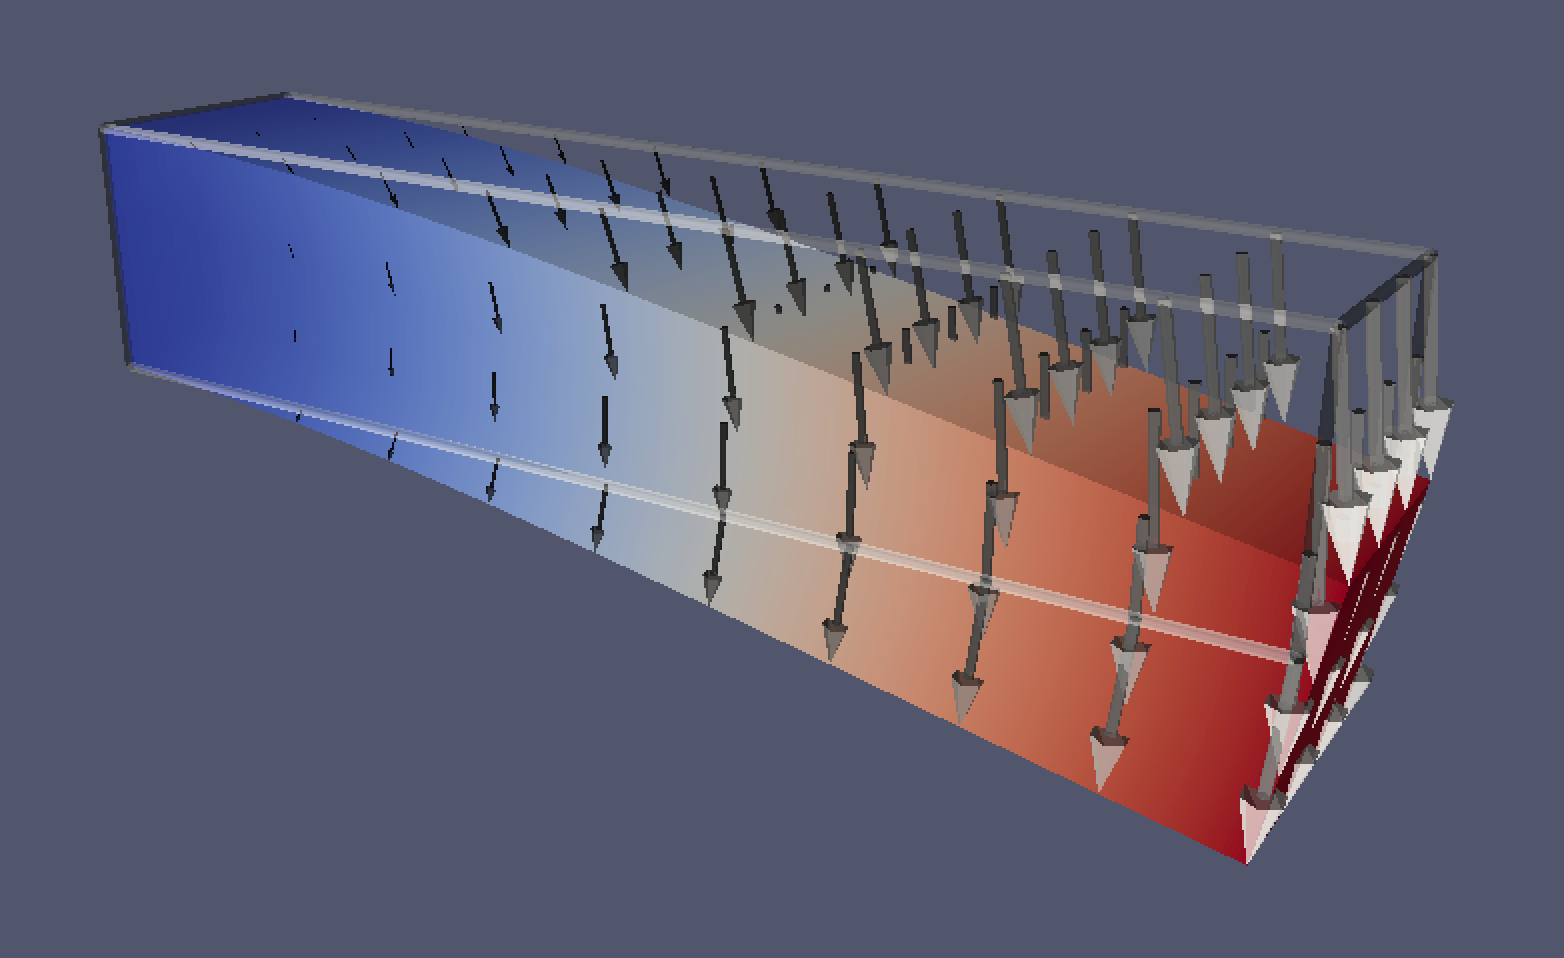
\includegraphics[width=0.95\linewidth]{fig/elasticity.png}}
%  \caption{
%  Plot of gravity-induced deflection in a clamped beam for the elasticity problem.
%  }
%\end{figure}

\section{Navier--Stokes方程}
\label{ftut1:NS}

\index{Navier-Stokes equations}
\index{CFD}

对于下一个例子,我们将解决不可压缩的Navier--Stokes
方程。 这个问题结合了我们的许多挑战
以前研究过的问题:时间依赖,非线性和
向量值变量。 我们将介绍一些FEniCS主题,
其中许多相当先进。 但你会看到,即使是相对的
复杂算法如二阶分割方法
不可压缩的Navier--Stokes方程,可以实现
FEniCS相对容易。

\subsection{PDE问题}

不可压缩的Navier--Stokes方程组成一个方程组
对于不可压缩流体的速度$u$和压力$p$:

\begin{align}
  \label{ftut1:ns:momentum}
  \varrho\left(\frac{\partial u}{\partial t} +
  u \cdot \nabla u\right) &= \nabla\cdot\sigma(u, p) + f, \\
  \label{ftut1:ns:continuity}
  \nabla \cdot u &= 0.
\end{align}
右边的$f$是每单位体积的给定力量
就线性弹性方程而言,
$\sigma(u,p)$表示应力张量,对于Newtonian流体
是(谁)给的

\index{stress tensor}

\begin{equation}
  \sigma(u, p) = 2\mu\epsilon(u) - pI,
\end{equation}
其中$\epsilon(u)$是应变率张量

\index{strain-rate tensor}

\[ \epsilon(u) = \frac{1}{2}\left(\nabla u + (\nabla u)^T\right)\tp\]
参数$\mu$是动态粘度。 注意势头
方程(\ref{ftut1:ns:momentum})非常类似于弹性
方程(\ref{ftut:elast:varform:equilibrium})。 区别在于
两个附加条款$\varrho(\partial u/ \partial t + u \cdot \ nabla u)$和不同的
表达式为应力张量。 两个额外的术语表达
加速平衡的力量$F = \nabla\cdot\sigma + f$每单位体积在Newton第二运动定律。

\subsection{变化公式}
\label{ftut1:NS:varform}

Navier--Stokes方程不同
我们需要解决一个系统的时间依赖热方程
方程式和这个系统是一种特殊的类型。 如果我们应用相同的
技术为热方程; 那就是更换时间
导数具有简单的差商,我们得到一个非线性
方程组。 这在
本身对于FEniCS来说不是一个问题,我们在第~\ref{ftut1:gallery:nonlinearpoisson}部分中看到,但系统有一个所谓的
\emph{saddle point structure},需要特殊技术
(特殊预处理器和迭代方法)有效解决。

\index{splitting method}
\index{Chorin's method}
\index{incremental pressure correction scheme}

相反,我们将应用一种更为简单和经常非常有效的方法,
称为\emph{splitting method}。 这个想法是
考虑两个方程(\ref{ftut1:ns:momentum})和
(\ref{ftut1:ns:continuity})。 存在许多分裂
不可压缩Navier--Stokes方程的策略。 其中一个
最古老的是由Chorin \cite{Chorin1968}提出的方法
Temam \cite{Temam1969},通常称为\emph{Chorin的方法}。 我们会
使用修改版本的Chorin的方法,即所谓的增量式
压力校正计划(IPCS)由于\cite{Goda1979}给出
与原来的方案相比,提高了准确度
成本。

IPCS方案涉及三个步骤。 首先,我们计算一个暂定的
速度$u^{\star}$通过推进动量方程
(\ref{ftut1:ns:momentum})通过中点有限差分方案
时间,但是使用压力$p^{n}$
以前的时间间隔。 我们还将线性化非线性对流
通过使用已知速度$u^{n}$从上一个时间步长:
$u^{n}\cdot\nabla u^{n}$。
第一步的变分问题是

\begin{align}
\label{ftut1:ipcs1}
      & \langle {\varrho(u^{\star} - u^{n}) / \dt},{v} \rangle
      + \langle {\varrho u^{n} \cdot \nabla u^{n}},{v} \rangle
      + \nonumber
        \langle {\sigma(u^{n+\frac{1}{2}}, p^{n})},{\epsilon(v)} \rangle \\
      &\quad\quad\quad\quad\quad
      + \langle {p^{n} n},{v} \rangle_{\partial\Omega}
      - \langle {\mu\nabla u^{n+\frac{1}{2}}\cdot n},{v} \rangle_{\partial\Omega}
      = \langle {f^{n+1}},{v} \rangle.
\end{align}
这种符号,适用于变化中许多术语的问题
配方,需要一些解释。 首先我们用短手
符号

\[
  \inner{v}{w} = \int_{\Omega} vw \dx, \quad
  \inner{v}{w}_{\partial\Omega} = \int_{\partial\Omega} vw \ds.
\]
这使我们能够更加紧凑地表达变分问题
办法。 其次,我们使用符号$u^{n +\frac{1}{2}}$。 这个符号
通常指的是间隔中点的$u$的值
近似于算术平均值:

\[
  u^{n+\frac{1}{2}} \approx (u^n + u^{n+1}) / 2.
\]
第三,我们注意到变分问题(\ref{ftut1:ipcs1})
源于该术语的部分整合
$\inner{-\nabla\cdot\sigma}{v}$。 就像弹性问题一样
段~\ref{ftut:elast},我们得到

\[
  \inner{-\nabla\cdot\sigma}{v}
  = \inner{\sigma}{\epsilon(v)}
  - \inner{T}{v}_{\partial\Omega},
\]
其中$T = \sigma\cdot n$是边界牵引力。如果我们解决了
有一个自由边界的问题,我们可以取$T = 0$
边界。但是,如果我们计算通过通道或管道的流量
并想要将持续进入“虚拟通道”的流模型化
外流,我们需要小心对待这个词。假设
那么我们就是制造出速度的方向导数
的通道在流出时为零,对应于流量
“完全发达”或者不显着下降
外流。这样做,流出的剩余边界就变成了
$pn - \mu\nabla u \cdot n$,这个术语出现在
变数问题(\ref{ftut1:ipcs1})。注意这个论点和
实现取决于$\nabla u$的确切定义
组件$\partial u_i / \partial x_j$或
$\partial u_j / \partial x_i$。我们这里选择后者,$\partial
u_j / \partial x_i$,这意味着我们必须使用FEniCS运算符
\verb!nabla_grad!为执行。如果我们使用\texttt{grad}运算符和
定义$\partial u_i / \partial x_j$,我们必须保留
条款$pn - \mu(\nabla u)^{\top} \cdot n$!

\index{grad@{\rm\texttt{grad}}}
\index{nabla\_grad@{\rm\texttt{nabla\_grad}}}

\begin{notice}%[\texttt{grad(u)} vs. \protect\verb!nabla\_grad(u)!]
对于标量函数,$\nabla u$具有清晰的含义作为向量

\[ \nabla u =\left(\frac{\partial u}{\partial x}, \frac{\partial u}{\partial y},
\frac{\partial u}{\partial z}\right)\tp\]
然而,如果$u$是向量值,则意义不太清楚。
一些源定义$\nabla u$作为具有元素的矩阵
$\partial u_j / \partial x_i$,而其他来源则喜欢
$\partial u_i / \partial x_j$。 在FEniCS中,\texttt{grad(u)}被定义为
矩阵与元素$\partial u_i / \partial x_j$,这是
$\nabla u$的自然定义,如果我们将其视为渐变或
$u$的衍生。 这样,可以应用矩阵$\nabla u$
一个差额$\dx$给出增量$\mathrm{d}u = \nabla u \,
\dx$。 因为$\nabla u$作为矩阵的替代解释
与元素$\partial u_j / \partial x_i$是非常常见的,in
特别在连续力学,FEniCS
提供操作员\verb!nabla_grad! 以此目的。
对于Navier-Stokes方程,重要的是考虑
术语$u \cdot \nabla u $应该被解释为向量
$w$与元素
$w_i = \sum_j \left(u_j \frac{\partial}{\partial x_j}\right) u_i
= \sum_j u_j \frac{\partial u_i}{\partial x_j}$。
这个术语可以在FEniCS中实现
\texttt{grad(u)*u},因为这是表达式
$\sum_j \partial u_i / \partial x_j u_j$,或as
\verb!dot(u,nabla_grad(u))! 因为这个表达式变成了
$\sum_i u_i \partial u_j / \partial x_i$。 我们将使用符号
\verb!dot(u,nabla_grad(u))! 以下,因为它更紧密地对应
到标准符号$u \cdot \nabla u$。

更准确地说,PDE有三种不同的符号
涉及梯度,发散和卷曲算子。一个雇用
$\mathrm{grad}\, u$,$\mathrm{div}\, u$和$\mathrm{curl}\, u$
运营商。另一个雇用$\nabla u$作为同义词
$\mathrm{grad}\, u$,$\nabla\cdot u$表示$\mathrm{div}\, u$和
$\nabla\times u$是$\mathrm{curl}\, u$的名称。第三
使用$\nabla u$,$\nabla\cdot u$和$\nabla\times u$
其中$\nabla$是\emph{vector},例如$\nabla u$是一个二进制
表达式:$(\nabla u)_{i,j} = \partial u_j/\partial x_i =
(\mathrm{grad}\,u)^{\top}$。后一个符号,以$\nabla$为一
向量运算符,在连续统计中得出方程时通常很方便
力学,如果这个解释$\nabla$是基础
你的PDE,你必须使用\verb!nabla_grad!, \verb!nabla_div!,和\verb!nabla_curl!在
FEniCS代码作为这些运算符兼容二进制
计算。从Navier--Stokes方程,我们可以很容易地看到
什么$\nabla$表示:如果对流术语的形式为$u \cdot
\nabla u$,实际上意思是$(u \cdot\nabla)u$,那么$\nabla$是
矢量和实现变成\verb!dot(u,nabla_grad(u))!在
FEniCS,但是如果我们看到$\nabla u\cdot u$或$(\mathrm{grad}u)\cdot u$,
相应的FEniCS表达式为\texttt{dot(grad(u),u)}。

类似地,张量场的发散如应力张量
$\sigma$也可以以两种不同的方式表达,或者
\texttt{div(sigma)}或\verb!nabla_div(sigma)! 第一种情况对应于
组件$\partial \sigma_ {ij}/{\partial x_j}$和第二个
$\partial \sigma_ {ij}/{\partial x_i}$。 一般来说,这些表达式
将会有所不同,但当压力测量是对称的时候
表达式具有相同的值。
\end{notice}

我们现在进入我们分裂计划的第二步
不可压缩的Navier--Stokes方程。 在第一步,我们计算
基于压力的初步速度$u^{\star}$
以前的时间步。 我们现在可以使用计算的暂定速度
计算新压力$p^n$:

\begin{equation}
\label{ftut1:ipcs2}
  \langle \nabla p^{n+1}, \nabla q \rangle
  = \langle {\nabla p^{n}},{\nabla q} \rangle
  - \dt^{-1} \langle{\nabla \cdot u^{\star}},{q} \rangle.
\end{equation}
请注意,$q$是压力的标量值测试函数
空间,而测试函数$v$在(\ref{ftut1:ipcs1})是一个
来自速度空间的向量值测试函数。

考虑这一步的一个方法是减去Navier--Stokes
动量方程(\ref{ftut1:ns:momentum})表示为
暂定速度$u^{\star}$和压力$p^n$来自
以速度$u^{n+1}$表示的动量方程
压力$p^{n+1}$。 这导致等式

\begin{equation} \label{ftut1:ipcs:step}
  (u^{n+1} - u^{\star}) / \dt + \nabla p^{n+1} - \nabla p^n = 0.
\end{equation}
采取分歧,并要求$\nabla \cdot u^{n+1} = 0$由
Navier--Stokes连续性方程(\ref{ftut1:ns:continuity}),我们
获得方程$-\nabla\cdot u^{\star} / \dt + \nabla^2 p^{n+1} -
\nabla^2 p^n = 0$,这是一个Poisson问题的压力$p^{n+1}$
导致变量问题(\ref{ftut1:ipcs2})。

最后,我们从公式计算出校正的速度$u^{n+1}$
(\ref{ftut1:ipcs:step})。 将该方程乘以测试函数
$v$,我们获得

\begin{equation}
\label{ftut1:ipcs3}
  \langle {u^{n+1}},{v} \rangle
  =
  \langle {u^{\star}},{v} \rangle
  - \dt \langle {\nabla(p^{n+1}-p^{n})},{v} \rangle.
\end{equation}

总而言之,我们可以解决不可压缩的Navier--Stokes
通过求解三个线性变分的序列有效地计算方程
每个时间步的问题。

\subsection{FEniCS实现}

\paragraph{测试问题1:通道流。}
\index{channel flow}

作为第一个测试问题,我们计算两个无限大的流量
板,所谓渠道或Poiseuille流。 我们将看到,这个
问题有一个已知的分析解决方案。 让$H$成为距离
盘间和$L$之间的通道长度。 没有
身体力量

\index{scaling}

我们可能首先扩大问题,摆脱看似独立的问题
物理参数。 这个问题的物理学是由
粘性效应仅在垂直于流动的方向,所以a
时间尺度应基于通道上的扩散: $t_c =
H^2/\nu$。 我们让$U$,一些特征流入速度是
速度尺度和$H$空间尺度。 采取压力秤
作为特征剪切应力,$\mu U/H$,因为这是主要的
剪切流动的例子。 插入$\bar x = x/H$,$\bar y = y/H$,
$\bar z = z/H$,$\bar u = u/U$,$\bar p = Hp/(\mu U)$,
方程式中的$\bar t = H^2/\nu$导致缩放的Navier-Stokes
方程式(缩放后的条形):

\index{Reynolds number}

\begin{align*}
\frac{\partial u}{\partial t} + \mathrm{Re}\, u\cdot\nabla u
&= -\nabla p + \nabla^2 u,\\
\nabla\cdot u &= 0\tp
\end{align*}

这里,$\mathrm{Re} = \varrho UH/\mu$是Reynolds数。 因为
的时间和压力尺度,这是不同的
对流主导的流体流量,Reynolds数量相关联
具有对流项,而不是粘度项。

通过假设$u=(u_x(x,y,z),0,0)$,得出确切的解
$x$轴指向通道。由于$\nabla\cdot u=0$,$u$
不能依赖$x$。渠道流动的物理学也是
二维,所以我们可以省略$z$坐标(更准确地说:
$\partial/\partial z=0$)。在(缩放)中插入$u=(u_x,0,0)$
控制方程式给出$u_x“(y) = \partial p/\partial x$。
相对于$x$区分这个方程式表示$\partial^2
p/\partial^2 x =0$ 所以 $\partial
p/\partial x$是一个常量,这里叫$-\beta$。这是开车
流量的力和可以指定为已知参数
问题。在通道的宽度上集成$u_x''(y)=-\beta$
$[0,1]$,并要求$u=(0, 0, 0)$在渠道墙,导致
$u_x=\frac{1}{2}\beta y(1-y)$。特征入口速度
$U$可以作为$y=1/2$的最大流入,意味着
$\beta = 8$。频道的长度,$L/H$在缩放
模型,对结果没有影响,所以为了简单,我们只是计算
在单位广场上。在数学上,必须规定压力
在某一点上,由于$p$不依赖于$y$,我们可以将$p$设置为a
沿着出口边界$x=1$的已知值,例如〜0。结果
是$p(x)=8(1-x)$和$u_x=4y(1-y)$。

边界条件可以设为$p=8$在$x=0$,$p=0$在$x=1$
和$u=(0, 0, 0)$在墙上$y=0,1$。 这定义了压降
并应导致入口和出口处的单位最大速度
抛物线速度曲线,无进一步规格。 注意
解决2D中的Navier--Stokes方程式是有意义的
3D几何,虽然潜在的数学问题崩溃了
到两个1D问题,一个用于$u_x(y)$,一个用于$p(x)$。

缩放模型不容易使用标准模拟
Navier--Stokes求解器。 但是,人们可以争辩说
对流项为零,所以这个术语前面的Re系数
在缩放的PDE中并不重要,可以设置为一致。 在那里面
在原始Navier-Stokes方程中设置$\varrho = \mu = 1$
类似于缩放模型。

对于具体的工程问题,想要模拟一个特定的
流体并设置相应的参数。因此,一般的解算器
最自然地实现与尺寸和原始的物理
参数。然而,缩放可以大大简化数值
模拟。首先,它表明所有的流体都在
同样的方式:我们是否有石油,天然气或水
两块板之间流动,流动速度无关紧要
是(达到某些批评价值的Reynolds号码的流量
变得不稳定并转变成复杂的湍流
完全不同的性质)。这意味着一个模拟就足够了
涵盖所有类型的渠道流程!在其他应用程序中,缩放
表明可能需要设置一些分数
参数(无量纲数)而不是参数
他们自己。这简化了探索输入参数空间
往往是模拟的目的。通常,缩放的问题是
通过将一些输入参数的尺寸设置为固定来运行
价值观(通常统一)。

\paragraph{FEniCS实现。}
我们以前的例子都是从创建网格开始的
然后在网格上定义一个\texttt{FunctionSpace}。 为了
Navier--Stokes分裂方案我们将需要定义两个函数
空间,一个为速度和一个为压力:

\begin{python}
V = VectorFunctionSpace(mesh, 'P', 2)
Q = FunctionSpace(mesh, 'P', 1)
\end{python}
第一个空格\texttt{V}是速度的向量值函数空间
而第二个空格\texttt{Q}是一个标量值的函数空间
压力。 我们使用分段二次元素作为速度
分段线性元件用于压力。 创建时
\texttt{VectorFunctionSpace}在FEniCS中,值维(的长度
向量)将被设置为等于该几何尺寸
有限元网格。 可以轻松创建向量值函数
通过添加关键字参数,FEniCS中的其他维度的空格
\texttt{dim}:

\index{VectorFunctionSpace@{\rm\texttt{VectorFunctionSpace}}}

\begin{python}
V = VectorFunctionSpace(mesh, 'P', 2, dim=10)
\end{python}

\begin{notice}[Navier--Stokes方程的稳定有限元空间]
众所周知,某些有限元空间不稳定
对于Navier--Stokes方程,或者甚至用于更简单的Stokes
方程。 有限元不稳定对的典型例子
空间是为了使用第一度连续分段多项式
速度和压力。 使用一个
不稳定的空间对通常会产生一个解决方案
虚假(想要的,非物理的)振荡的压力
解。 简单的补救办法是连续使用
速度和连续分段线性的二次元素
元素为压力。 这些元素一起形成所谓的
\emph{Taylor-Hood}元素。 杂散振荡也可能发生
如果使用不稳定的元素对,则可以使用拆分方法。
\end{notice}

由于我们有两个不同的函数空间,我们需要创建两个集合
的试用和测试功能:

\begin{python}
u = TrialFunction(V)
v = TestFunction(V)
p = TrialFunction(Q)
q = TestFunction(Q)
\end{python}

\index{near@{\rm\texttt{near}}}

正如我们在前面的例子中所看到的,边界可能被定义在
FEniCS通过定义返回\texttt{True}或\texttt{False}的Python函数
取决于一个点是否应该被视为一部分
边界

\begin{python}
def boundary(x, on_boundary):
    return near(x[0], 0)
\end{python}
该函数定义了所有点的边界
$x$- 坐标等于接近零。 \texttt{near}函数来自
FEniCS并执行公差测试:\texttt{abs(x[0] - 0) < 3E-16}所以我们
不要遇到烦恼。 或者,我们可以给
边界定义作为一个字符串的C++代码,很像我们有
先前定义的表达式,如
\verb!u_D = Expression('1 + x[0]*x[0] + 2*x[1]*x[1]',degree=2)!。
上述边界的定义Python函数的术语可能由简单的C ++代替串:

\begin{python}
boundary = 'near(x[0], 0)'
\end{python}
这具有移动哪些节点的计算的优点
属于从Python到C++的边界,这提高了效率
的程序。

对于当前的例子,我们将设置三个不同的边界
条件。 首先,我们将在通道的墙壁设置$u = 0$;
也就是说,在$y = 0$和$y = 1$。 其次,我们将设置$p = 8$
流入($x = 0$),最后流出$p = 0$ ($x = 1$)。 这个
将导致压力梯度,从而加速流动
零速度的初始状态。 这些边界条件可能是
定义如下:

\begin{python}
# Define boundaries
inflow   = 'near(x[0], 0)'
outflow  = 'near(x[0], 1)'
walls    = 'near(x[1], 0) || near(x[1], 1)'

# Define boundary conditions
bcu_noslip  = DirichletBC(V, Constant((0, 0)), walls)
bcp_inflow  = DirichletBC(Q, Constant(8), inflow)
bcp_outflow = DirichletBC(Q, Constant(0), outflow)
bcu = [bcu_noslip]
bcp = [bcp_inflow, bcp_outflow]
\end{python}

最后,我们收集速度的边界条件
Python列表中的压力,所以我们可以轻松访问它们
以下计算。

我们现在转向变分形式的定义。 有
要定义三个变量问题,一个为每个步骤
IPCS方案。 我们来看一下第一个变分的定义
问题。 我们从一些常数开始:

\begin{python}
U   = 0.5*(u_n + u)
n   = FacetNormal(mesh)
f   = Constant((0, 0))
k   = Constant(dt)
mu  = Constant(mu)
rho = Constant(rho)
\end{python}

下一步是设置第一步的变分形式
(\ref{ftut1:ipcs1})。 由于变异
问题包含已知和未知数量的混合,我们将使用
以下命名约定:\texttt{u}是未知数(数学上
$u^{n+1}$)作为变体形式的试用函数,\verb!u_! 是个
最近计算的近似值($u^{n+1}$可用作为
\texttt{Function}对象),\verb!u_n! 是$u^n$,同样的约定
\texttt{p},\verb!p_! ($p^{n+1}$)和\verb!p_n!($P^N$)。

\begin{python}
# Define strain-rate tensor
def epsilon(u):
    return sym(nabla_grad(u))

# Define stress tensor
def sigma(u, p):
    return 2*mu*epsilon(u) - p*Identity(len(u))

# Define variational problem for step 1
F1 = rho*dot((u - u_n) / k, v)*dx + \
     rho*dot(dot(u_n, nabla_grad(u_n)), v)*dx \
   + inner(sigma(U, p_n), epsilon(v))*dx \
   + dot(p_n*n, v)*ds - dot(mu*nabla_grad(U)*n, v)*ds \
   - dot(f, v)*dx
a1 = lhs(F1)
L1 = rhs(F1)
\end{python}

请注意,我们利用Python编程语言
定义我们自己的运算符\texttt{sigma}和\texttt{epsilon}。 以这种方式使用Python
可以轻松扩展FEniCS的数学语言
特殊经营者和组织法。

还要注意,FEniCS可以整理双线性形式$a(u,v)$和
线性形式$L(v)$形式由\texttt{lhs}
和\texttt{rhs}函数。 这在更长的时间里是特别方便的
更复杂的变化形式。

分裂方案需要解决三个序列
变化问题在每个时间步。 我们以前用过了
内置的FEniCS函数\texttt{solve}来解决变分问题。 下
引擎盖,当用户调用\texttt{solve(a == L,u,bc)}时,FEniCS会
执行以下步骤:

\begin{python}
A = assemble(A)
b = assemble(L)
bc.apply(A, b)
solve(A, u.vector(), b)
\end{python}
在最后一步中,FEniCS使用重载的\texttt{solve}函数来解决
线性系统\texttt{AU = b}其中\texttt{U}是度的向量
函数的自由$u(x) = \sum_{j=1} U_j \phi_j(x)$。

\index{linear system}

在执行分裂计划时,我们将利用
这些低级命令首先组装然后调用解决。 这个
具有我们可以控制何时组装和我们的优势
解决线性系统。 特别是,由于矩阵为
三个变数问题都是时间无关的,这是有道理的
在时间循环之外组合它们一次:

\index{assemble@{\rm\texttt{assemble}}}

\begin{python}
A1 = assemble(a1)
A2 = assemble(a2)
A3 = assemble(a3)
\end{python}
在时间步进循环中,我们然后可以组装
右侧向量,应用边界条件,并调用求解
功能如下这三个步骤中的第一步:

\begin{python}
# Time-stepping
t = 0
for n in range(num_steps):

    # Update current time
    t += dt

    # Step 1: Tentative velocity step
    b1 = assemble(L1)
    [bc.apply(b1) for bc in bcu]
    solve(A1, u_.vector(), b1)
\end{python}
注意在bcu中的bc的Python \emph{list comprehension} \texttt{[bc.apply(b1)]}
它遍历列表\texttt{bcu}中的所有\texttt{bc}。 这是一个方便
和紧凑的方式来构建一个适用的循环
所有边界条件在一条线上。 此外,代码工作如果
我们在未来添加更多的Dirichlet边界条件。 注意
边界条件只需要应用于右边
向量,因为它们已经被应用于矩阵(未示出)。

最后,我们来看一下我们如何使用参数的重要细节
例如我们变分的定义中的时间步长\texttt{dt}
问题。 因为我们以后可能想改变这些,例如,如果我们
想要尝试更小或更大的时间步骤,我们包装这些
使用FEniCS \texttt{Constant}:

\begin{python}
k = Constant(dt)
\end{python}

FEniCS中的矩阵和向量的汇编基于代码
代。 这意味着每当我们改变一个变数问题时,
FENiCS将必须生成新的代码,这可能需要一点时间
时间。 新的代码也将生成和编译时的浮点值
因为时间的改变。 通过使用此参数包装
\texttt{Constant},FEniCS将把该参数视为通用常量
不是一个特定的数值,它可以防止重复的代码
代。 在时间步长的情况下,我们选择一个新的名字\texttt{k}
而不是\texttt{dt}为\texttt{Constant},因为我们也想使用
变量\texttt{dt}作为Python float作为时间步长的一部分。

用于使用FEniCS模拟2D通道流的完整代码
可以在文件中找到
\begin{center}
  \url{https://fenicsproject.org/pub/tutorial/python/vol1/ft07_navier_stokes_channel.py}
\end{center}
\begin{center}
  \nolinkurl{ft07_navier_stokes_channel.py}。
\end{center}

\index{ft07\_navier\_stokes\_channel.py@{\rm\texttt{ft07\_navier\_stokes\_channel.py}}}

\paragraph{验证。}
\index{verification}

我们计算节点上的错误,就像我们之前做过的那样来验证
我们的实施是正确的。 我们的Navier--Stokes求解器计算
解决时间依赖的不可压缩Navier--Stokes
方程式,从初始条件$u =(0, 0)$开始。 我们有
没有在我们的求解器中明确指定初始条件
意味着FEniCS将初始化所有变量,特别是
以前的和当前的速度\verb!u_n! 和\verb!u_!,为零。 自从
精确解是二次的,我们期望解决方案是准确的
在无限时间的节点处的机器精度。 对于我们
实现时,错误快速接近零,大约为零
$10^{-6}$在时间$T = 10$。

%\begin{figure}[!ht]  % ftut1:fig:navier_stokes_channel
%  \centerline{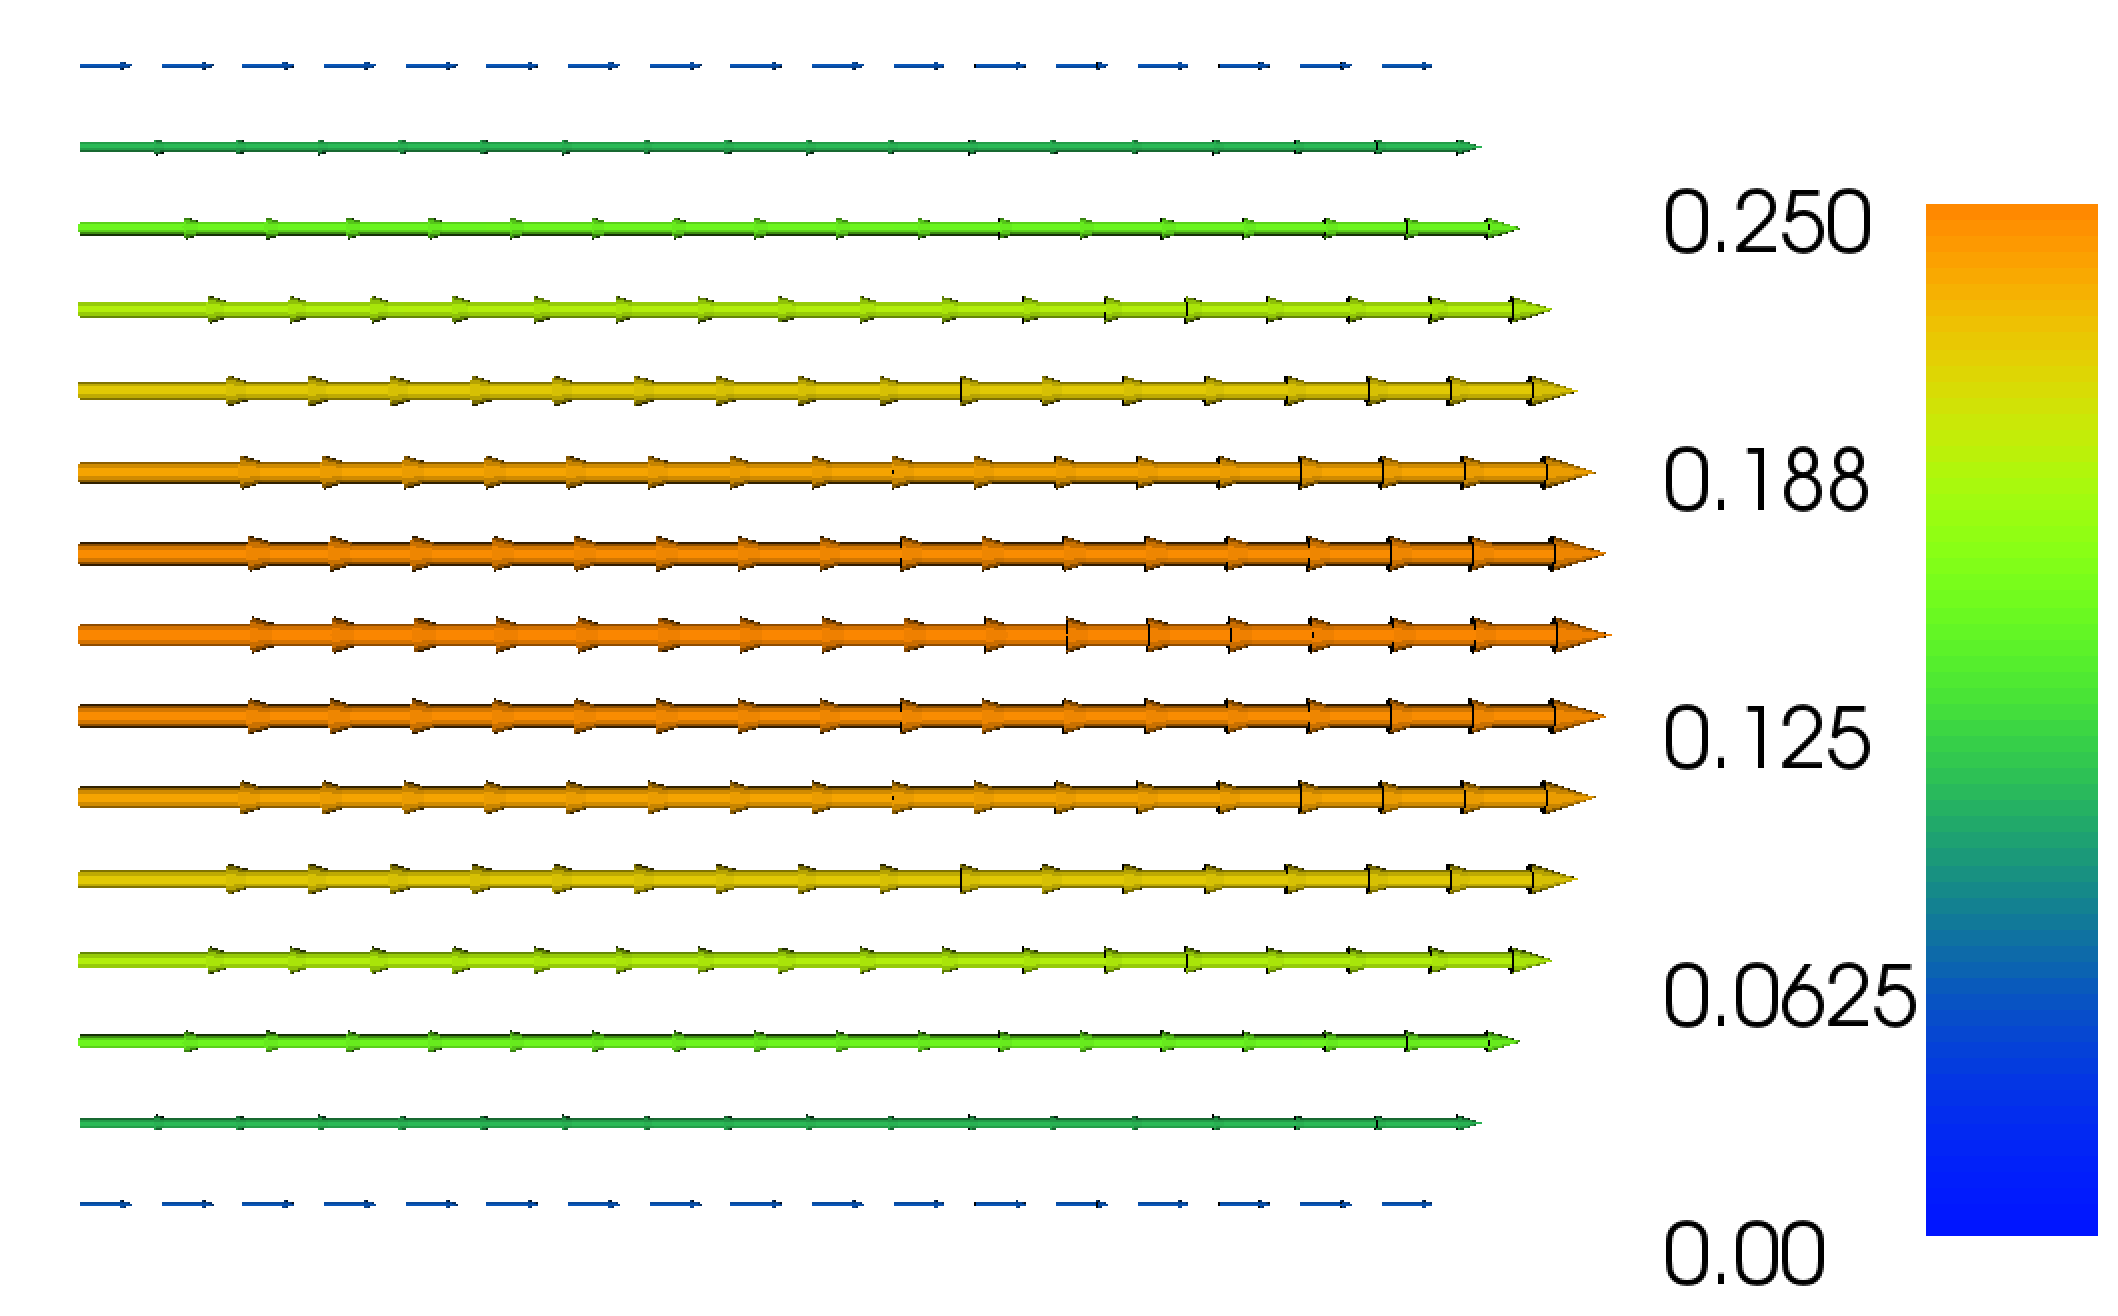
\includegraphics[width=0.95\linewidth]{fig/navier_stokes_channel.png}}
%  \caption{
%  Plot of the velocity profile at the final time for the Navier--Stokes channel flow example. \label{ftut1:fig:navier_stokes_channel}
%  }
%\end{figure}

\paragraph{测试问题2:流过气瓶。}
\index{cylinder flow}

现在我们把注意力转向一个更具挑战性的问题:流程
经过一个圆柱体。 几何和参数取自
问题DFG 2D-2在\url{http://www.featflow.de/en/benchmarks/cfdbenchmarking/flow/dfg_benchmark2_re100.html}{FEATFLOW/1995-DFG benchmark suite}\footnote{\texttt{http://www.featflow.de/en/benchmarks/cfdbenchmarking/flow/dfg\_benchmark2\_re100.html}}
并且如图~\ref{ftut1:navier_stokes_cylinder:geometry}所示。 运动粘度为
由$\nu = 0.001 = \mu/\varrho$给出,流入速度分布为
指定为

\[
  u(x, y, t) = \left(1.5 \cdot \frac{4y(0.41 - y)}{0.41^2}, 0\right),
\]
其最大幅度为$1.5$,$y = 0.41/2$。 我们不
使用任何缩放来解决这个问题,因为所有的精确参数都是已知的。

%\begin{figure}[!ht]  % ftut1:navier_stokes_cylinder:geometry
%  \centerline{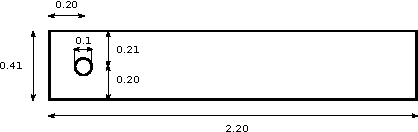
\includegraphics[width=0.95\linewidth]{fig/navier_stokes_cylinder_geometry.pdf}}
%  \caption{
%  Geometry for the flow past a cylinder test problem. Notice the slightly perturbed and unsymmetric geometry. \label{ftut1:navier_stokes_cylinder:geometry}
%  }
%\end{figure}

\paragraph{FEniCS实现。}
到目前为止,我们所有的领域都是简单的形状,如单位面积或
一个矩形盒子。 可以创建许多这样简单的网格
在FEniCS中使用内置的网格类
(\texttt{UnitIntervalMesh},
\texttt{UnitSquareMesh},
\texttt{UnitCubeMesh},
\texttt{IntervalMesh},
\texttt{RectangleMesh},
\texttt{BoxMesh})。
FEniCS支持通过技术创建更复杂的网格
称为\emph{constructive solid geometry}(CSG),这使我们可以定义
几何形状简单的形状(基元)和设置操作:
联合,交集和设置差异。 设置操作是
使用运算符\texttt{+}(联盟),\texttt{*}(交集)在FEniCS中编码,
和\texttt{-}(设置差异)。 要访问FEniCS中的CSG功能,
必须导入提供的FEniCS模块\texttt{mshr}
FEniCS的扩展网格划分功能。

\index{mshr}
\index{CSG}
\index{constructive solid geometry}

气缸流量测试问题的几何可以很容易地定义
通过首先定义矩形通道,然后减去
圈:

\begin{python}
channel = Rectangle(Point(0, 0), Point(2.2, 0.41))
cylinder = Circle(Point(0.2, 0.2), 0.05)
domain = channel - cylinder
\end{python}
然后我们可以通过调用函数\verb!generate_mesh!创建网格:

\begin{python}
mesh = generate_mesh(domain, 64)
\end{python}
这里的参数\texttt{64}表示我们要解决几何
其直径为64个(通道长度)。

\index{generate\_mesh@{\rm\texttt{generate\_mesh}}}

为了解决缸体测试问题,我们只需要做一些次要的
更改我们为通道流测试编写的代码
案件。 除了定义新的网格,我们需要做出的唯一的改变
是修改边界条件和时间步长。该
边界规定如下:

\begin{python}
inflow   = 'near(x[0], 0)'
outflow  = 'near(x[0], 2.2)'
walls    = 'near(x[1], 0) || near(x[1], 0.41)'
cylinder = 'on_boundary && x[0]>0.1 && x[0]<0.3 && x[1]>0.1 && x[1]<0.3'
\end{python}
最后一行可能看起来似乎是隐秘的,然后才能抓住这个想法:我们想选择
出现也位于x2D内的所有边界点(\verb!on_boundary!)
域$[0.1,0.3]\times [0.1,0.3]$,参见图~\ref{ftut1:navier_stokes_cylinder:geometry}。
唯一可能的点就是这些点
循环边界!

\index{set\_log\_level@{\rm\texttt{set\_log\_level}}}
\index{DEBUG@{\rm\texttt{DEBUG}} log level}
\index{PROGRESS@{\rm\texttt{PROGRESS}} log level}

除了这些重要的变化,我们还会做一些小的
改变我们的解决方案。 首先,因为我们需要选择一个
相对较小的时间步长来计算解决方案(一个时间步长
太大会使解决方案爆炸)我们添加了一个进度条
我们可以跟随我们的计算进度。 这可以做到
如下:

\index{Progress@{\rm\texttt{Progress}}}

\begin{python}
progress = Progress('Time-stepping')
set_log_level(PROGRESS)

# Time-stepping
t = 0.0
for n in range(num_steps):

    # Update current time
    t += dt

    # Place computation here

    # Update progress bar
    progress.update(t / T)
\end{python}

\begin{notice}[日志级别和FEniCS中的打印]
注意调用\verb!set_log_level(PROGRESS)! 这是至关重要的
使FEniCS实际显示进度条。 FEniCS其实是
相当丰富的信息,在计算过程中发生了什么
打印到屏幕的信息量取决于当前日志
水平。 只有优先级高于或等于的消息
将显示当前日志级别。 预定义的日志级别
FEniCS是
\texttt{DBG},
\texttt{TRACE},
\texttt{PROGRESS},
\texttt{INFO},
\texttt{WARNING},
\texttt{ERROR},和
\texttt{CRITICAL}。默认情况下,日志级别设置为\texttt{INFO}
级别为\texttt{DBG},\texttt{TRACE}和\texttt{PROGRESS}的邮件不会
打印。 用户可以使用FEniCS功能\texttt{info}打印消息,
\texttt{warning}和\texttt{error},它将在明显的日志中打印消息
级别(在\texttt{error}的情况下也会抛出异常
出口)。 也可以使用呼叫 \texttt{log(level,message)}来打印
消息在特定日志级别。
\end{notice}

由于线性方程组的系统明显大于
对于简单的通道流量测试问题,我们选择使用
迭代方法而不是使用的默认直接(稀疏)求解器
调用\texttt{solve}时的FEniCS。 线性系统的有效解决方案
由PDEs的离散化产生的,需要选择a
良好的迭代(Krylov子空间)方法和良好的
预条件。 对于这个问题,我们将简单地使用双共轭
梯度稳定法(BiCGSTAB)和共轭梯度法。 这可以通过添加来完成
在\texttt{solve}的调用中,关键字\texttt{bicgstab}或\texttt{cg}。 我们也指定
适当的预处理器来加速计算:

\index{Krylov solver}
\index{preconditioner}

\begin{python}
solve(A1, u1.vector(), b1, 'bicgstab', 'hypre_amg')
solve(A2, p1.vector(), b2, 'bicgstab', 'hypre_amg')
solve(A3, u1.vector(), b3, 'cg', 'sor')
\end{python}

最后,为了能够在ParaView中对计算出的解决方案进行后处理,
我们将解决方案存储在每个时间步长中的文件中。 我们以前
为此,使用后缀\texttt{.pvd}创建文件。 在例子中
程序
\url{https://fenicsproject.org/pub/tutorial/python/vol1/ft04_heat_gaussian.py}{\nolinkurl{ft04_heat_gaussian.py}},
我们首先创建一个名为\verb!heat_gaussian/solution.pvd!的文件 接着
在每个时间步骤中保存解决方案
\begin{python}
vtkfile << (u, t)
\end{python}

对于本示例,我们将选择保存解决方案
到XDMF格式。 此文件格式与\texttt{.pvd}文件类似
我们以前看过但有几个优点。 首先,存储是
在速度和文件大小方面都更有效率。 第二,
\texttt{.xdmf}文件可以并行工作,无论是写作还是阅读
(后期处理)。 很像\texttt{.pvd}文件,实际数据将不会
存储在\texttt{.xdmf}文件本身,而是存储在一个
(单个)单独的数据文件与后缀\texttt{.hdf5}是一个
专为高性能计算设计的高级文件格式。
我们创建XDMF文件如下:

\begin{python}
xdmffile_u = XDMFFile('navier_stokes_cylinder/velocity.xdmf')
xdmffile_p = XDMFFile('navier_stokes_cylinder/pressure.xdmf')
\end{python}
在每个时间步骤中,我们可以存储速度和压力
\begin{python}[language=Python,style=graycolor]
xdmffile_u.write(u, t)
xdmffile_p.write(p, t)
\end{python}

\index{TimeSeries@{\rm\texttt{TimeSeries}}}
\index{HDF5 format}
\index{XDMF format}
\index{.hdf5@{\rm\texttt{.hdf5}} file}
\index{.xdmf@{\rm\texttt{.xdmf}} file}

我们还使用FEniCS \texttt{TimeSeries}存储解决方案。 这让我们
存储解决方案不是为了可视化,而是为了稍后重用
计算,我们将在下一节中看到。 使用\texttt{TimeSeries}
从某些方面阅读解决方案是很容易和有效的
模拟期间的时间。 \texttt{TimeSeries}类也使用HDF5
用于高效存储和访问数据的文件格式。

图~\ref{ftut1:fig:navier_stokes_cylinder:velocity}和~\ref{ftut1:fig:navier_stokes_cylinder:pressure}显示速度和
最终时间的压力在ParaView中可视化。 对于可视化
的速度,我们使用\textbf{Glyph}过滤器来可视化
矢量速度场。 为了可视化的压力,我们有
使用\textbf{Warp By Scalar}过滤器。

%\begin{figure}[!ht]  % ftut1:fig:navier_stokes_cylinder:velocity
%  \centerline{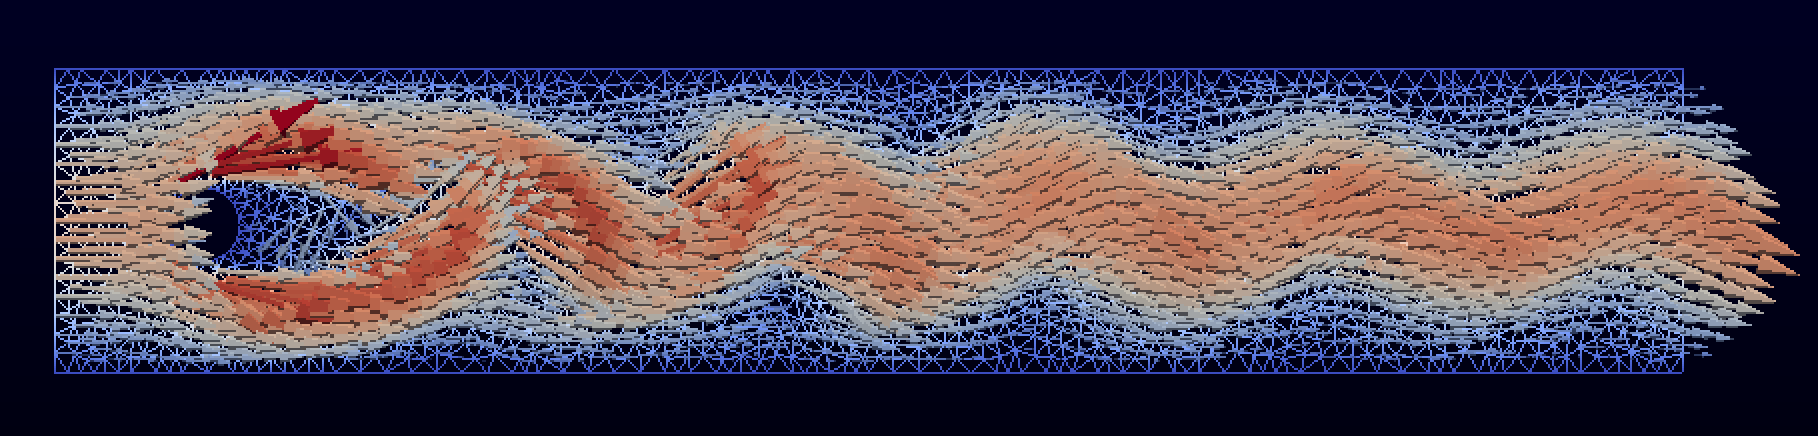
\includegraphics[width=0.95\linewidth]{fig/navier_stokes_cylinder_velocity.png}}
%  \caption{
%  Plot of the velocity for the cylinder test problem at final time. \label{ftut1:fig:navier_stokes_cylinder:velocity}
%  }
%\end{figure}

%\begin{figure}[!ht]  % ftut1:fig:navier_stokes_cylinder:pressure
%  \centerline{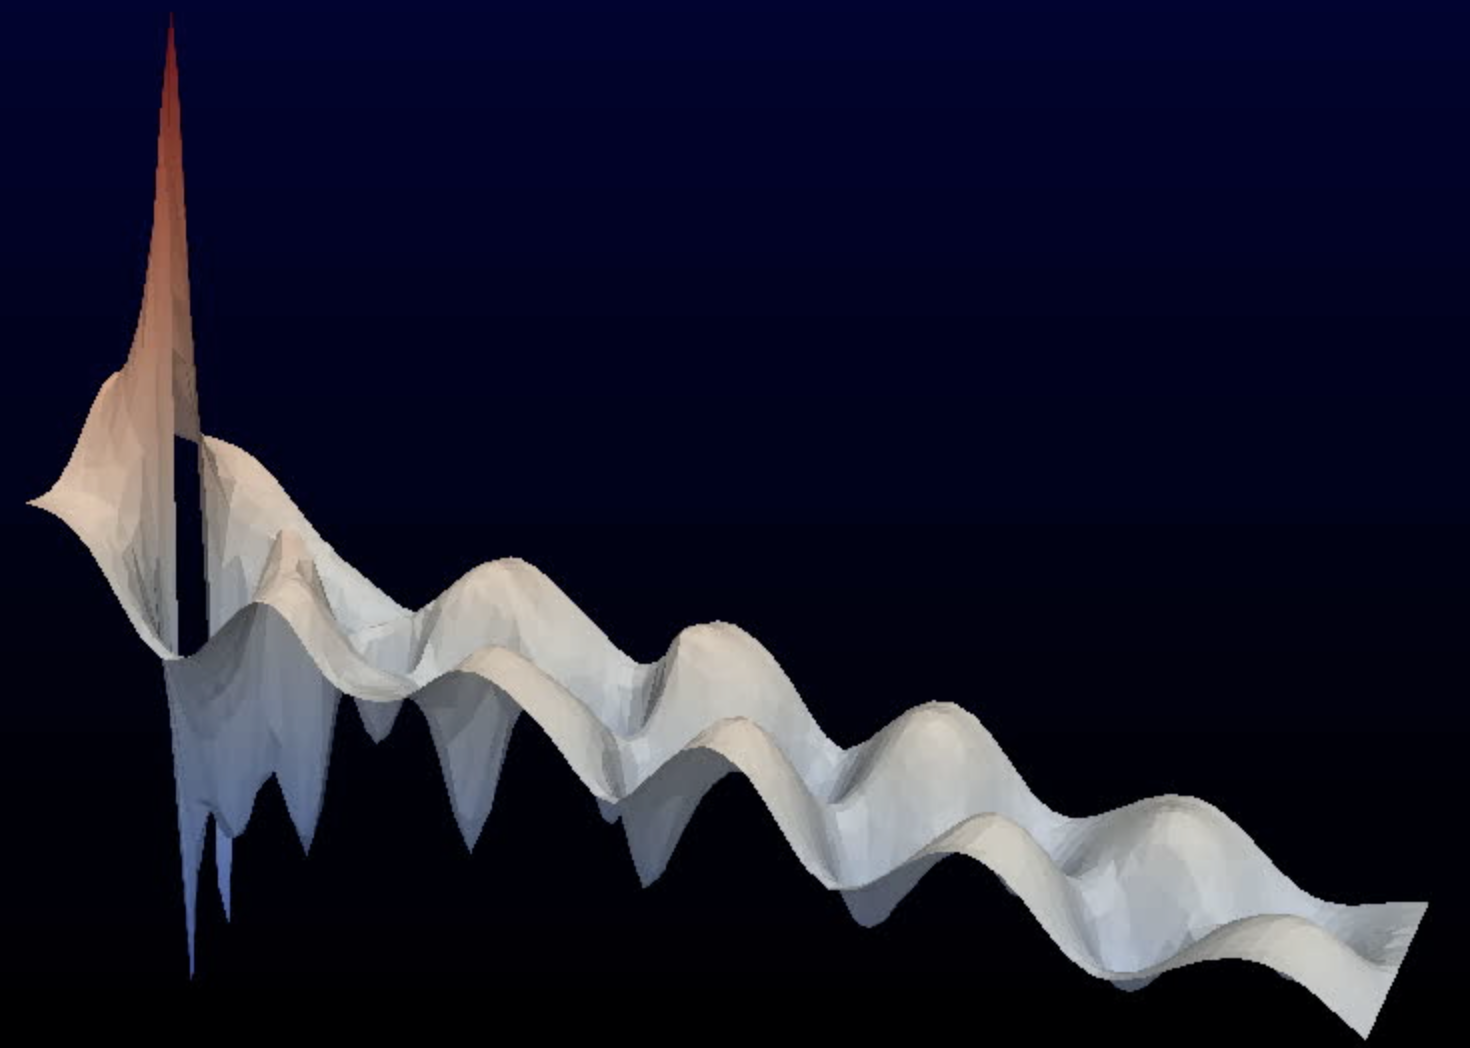
\includegraphics[width=0.95\linewidth]{fig/navier_stokes_cylinder_pressure.png}}
%  \caption{
%  Plot of the pressure for the cylinder test problem at final time. \label{ftut1:fig:navier_stokes_cylinder:pressure}
%  }
%\end{figure}

气缸测试问题的完整代码看起来像
如下:

\begin{python}
from fenics import *
from mshr import *
import numpy as np

T = 5.0            # final time
num_steps = 5000   # number of time steps
dt = T / num_steps # time step size
mu = 0.001         # dynamic viscosity
rho = 1            # density

# Create mesh
channel = Rectangle(Point(0, 0), Point(2.2, 0.41))
cylinder = Circle(Point(0.2, 0.2), 0.05)
domain = channel - cylinder
mesh = generate_mesh(domain, 64)

# Define function spaces
V = VectorFunctionSpace(mesh, 'P', 2)
Q = FunctionSpace(mesh, 'P', 1)

# Define boundaries
inflow   = 'near(x[0], 0)'
outflow  = 'near(x[0], 2.2)'
walls    = 'near(x[1], 0) || near(x[1], 0.41)'
cylinder = 'on_boundary && x[0]>0.1 && x[0]<0.3 && x[1]>0.1 && x[1]<0.3'

# Define inflow profile
inflow_profile = ('4.0*1.5*x[1]*(0.41 - x[1]) / pow(0.41, 2)', '0')

# Define boundary conditions
bcu_inflow = DirichletBC(V, Expression(inflow_profile, degree=2), inflow)
bcu_walls = DirichletBC(V, Constant((0, 0)), walls)
bcu_cylinder = DirichletBC(V, Constant((0, 0)), cylinder)
bcp_outflow = DirichletBC(Q, Constant(0), outflow)
bcu = [bcu_inflow, bcu_walls, bcu_cylinder]
bcp = [bcp_outflow]

# Define trial and test functions
u = TrialFunction(V)
v = TestFunction(V)
p = TrialFunction(Q)
q = TestFunction(Q)

# Define functions for solutions at previous and current time steps
u_n = Function(V)
u_  = Function(V)
p_n = Function(Q)
p_  = Function(Q)

# Define expressions used in variational forms
U  = 0.5*(u_n + u)
n  = FacetNormal(mesh)
f  = Constant((0, 0))
k  = Constant(dt)
mu = Constant(mu)
rho = Constant(rho)

# Define symmetric gradient
def epsilon(u):
    return sym(nabla_grad(u))

# Define stress tensor
def sigma(u, p):
    return 2*mu*epsilon(u) - p*Identity(len(u))

# Define variational problem for step 1
F1 = rho*dot((u - u_n) / k, v)*dx \
   + rho*dot(dot(u_n, nabla_grad(u_n)), v)*dx \
   + inner(sigma(U, p_n), epsilon(v))*dx \
   + dot(p_n*n, v)*ds - dot(mu*nabla_grad(U)*n, v)*ds \
   - dot(f, v)*dx
a1 = lhs(F1)
L1 = rhs(F1)

# Define variational problem for step 2
a2 = dot(nabla_grad(p), nabla_grad(q))*dx
L2 = dot(nabla_grad(p_n), nabla_grad(q))*dx - (1/k)*div(u_)*q*dx

# Define variational problem for step 3
a3 = dot(u, v)*dx
L3 = dot(u_, v)*dx - k*dot(nabla_grad(p_ - p_n), v)*dx

# Assemble matrices
A1 = assemble(a1)
A2 = assemble(a2)
A3 = assemble(a3)

# Apply boundary conditions to matrices
[bc.apply(A1) for bc in bcu]
[bc.apply(A2) for bc in bcp]

# Create XDMF files for visualization output
xdmffile_u = XDMFFile('navier_stokes_cylinder/velocity.xdmf')
xdmffile_p = XDMFFile('navier_stokes_cylinder/pressure.xdmf')

# Create time series (for use in reaction_system.py)
timeseries_u = TimeSeries('navier_stokes_cylinder/velocity_series')
timeseries_p = TimeSeries('navier_stokes_cylinder/pressure_series')

# Save mesh to file (for use in reaction_system.py)
File('navier_stokes_cylinder/cylinder.xml.gz') << mesh

# Create progress bar
progress = Progress('Time-stepping')
set_log_level(PROGRESS)

# Time-stepping
t = 0
for n in range(num_steps):

    # Update current time
    t += dt

    # Step 1: Tentative velocity step
    b1 = assemble(L1)
    [bc.apply(b1) for bc in bcu]
    solve(A1, u_.vector(), b1, 'bicgstab', 'hypre_amg')

    # Step 2: Pressure correction step
    b2 = assemble(L2)
    [bc.apply(b2) for bc in bcp]
    solve(A2, p_.vector(), b2, 'bicgstab', 'hypre_amg')

    # Step 3: Velocity correction step
    b3 = assemble(L3)
    solve(A3, u_.vector(), b3, 'cg', 'sor')

    # Plot solution
    plot(u_, title='Velocity')
    plot(p_, title='Pressure')

    # Save solution to file (XDMF/HDF5)
    xdmffile_u.write(u_, t)
    xdmffile_p.write(p_, t)

    # Save nodal values to file
    timeseries_u.store(u_.vector(), t)
    timeseries_p.store(p_.vector(), t)

    # Update previous solution
    u_n.assign(u_)
    p_n.assign(p_)

    # Update progress bar
    progress.update(t / T)
    print('u max:', u_.vector().array().max())

# Hold plot
interactive()
\end{python}
该程序可以在文件\url{https://fenicsproject.org/pub/tutorial/python/vol1/ft08_navier_stokes_cylinder.py}{\nolinkurl{ft08_navier_stokes_cylinder.py}}中找到。
应该告诉读者,这个例子程序很大
比我们以前的例子在CPU时间和要求更高
记忆,但应该可以合理地运行程序
现代笔记本电脑。

\index{ft08\_navier\_stokes\_cylinder.py@{\rm\texttt{ft08\_navier\_stokes\_cylinder.py}}}

\section{平流--扩散--反应方程组}
\label{ftut1:reactionsystem}

\index{advection--diffusion--reaction}
\index{chemical reactions}
\index{reaction system}

到目前为止我们遇到的问题 - 有显着的例外
的Navier--Stokes方程 - 都有一个共同的特征:它们都是
涉及由单个标量或向量PDE表达的模型。 在很多
情况下,模型被表示为PDE系统,
描述可能由(非常)不同的管理的不同数量
物理。 正如我们所看到的Navier-Stokes方程式,一种解决方法
FEniCS中的PDE系统是使用我们解决的分割方法
一个方程,并将解从一个方程提供给
下一个。 然而,FEniCS的优势之一是轻松
哪一个可以代替几个相互联系的变分问题
PDE成为一个复合系统。 在本节中,我们将介绍如何使用
FEniCS为这种耦合PDE系统写出求解器。
目标是展示实现完全隐含的容易程度,
在FEniCS中也称为单片,求解器。

\index{coupled systems}

\subsection{PDE问题}

我们的模型问题是以下系统
平流--扩散--反应方程:

\begin{align}
  \label{ftut1:reactionsystem:system:1}
  \frac{\partial u_1}{\partial t} +
  w \cdot \nabla u_1 - \nabla\cdot(\epsilon\nabla u_1)
    &= f_1 -K u_1 u_2, \\
  \label{ftut1:reactionsystem:system:2}
  \frac{\partial u_2}{\partial t} +
  w \cdot \nabla u_2 - \nabla\cdot(\epsilon\nabla u_2)
    &= f_2 -K u_1 u_2, \\
  \label{ftut1:reactionsystem:system:3}
  \frac{\partial u_3}{\partial t} +
  w \cdot \nabla u_3 - \nabla\cdot(\epsilon\nabla u_3)
    &= f_3 + K u_1 u_2 - K u_3.
\end{align}

该系统模拟两种物质之间的化学反应$A$和
$B$在某些域$\Omega$:

\[
  A + B \rightarrow C.
\]

我们假设反应是\emph{first-order},意思是
反应速率与浓度$[A]$和$[B]$成正比
两种物品$A$和$B$:

\[
  \frac{\mathrm{d}}{\mathrm{d}t} [C] = K [A] [B].
\]
我们还假设形成的物种$C$自发衰减
速率与浓度成比例$[C]$。 在PDE系统中
(\ref{ftut1:reactionsystem:system:1})--(\ref{ftut1:reactionsystem:system:3}),
我们使用变量$u_1$,$u_2$和$u_3$来表示
三种物种的浓度:

\[
  u_1 = [A], \quad u_2 = [B], \quad u_3 = [C].
\]
我们看到化学反应是在
PDE系统的右侧(\ref{ftut1:reactionsystem:system:1})--(\ref{ftut1:reactionsystem:system:3})。

化学反应参与域中的每个点
$\Omega$。 此外,我们假设物种$A$,$B$和$C$
在整个域扩散扩散性$\epsilon$(术语
$-\nabla\cdot(\epsilon\nabla u_i)$),并以速度平缓
$w$(术语$w\cdot\nabla u_i$)。

为了使事物的视觉和身体感兴趣,我们将让它
化学反应发生在从中计算出的速度场
解决不可压缩的Navier--Stokes方程
圆柱体从上一节。 总而言之,我们将会是
求解以下非线性PDE耦合系统:

\begin{align}
  \label{ftut1:reactionsystem:full}
  \varrho\left(\frac{\partial w}{\partial t} +
  w \cdot \nabla w\right) &= \nabla\cdot\sigma(w, p) + f, \\
  \nabla \cdot w &= 0, \\
  \frac{\partial u_1}{\partial t} +
  w \cdot \nabla u_1 - \nabla\cdot(\epsilon\nabla u_1)
    &= f_1 - K u_1 u_2, \\
  \frac{\partial u_2}{\partial t} +
  w \cdot \nabla u_2 - \nabla\cdot(\epsilon\nabla u_2)
    &= f_2 - K u_1 u_2, \\
  \frac{\partial u_3}{\partial t} +
  w \cdot \nabla u_3 - \nabla\cdot(\epsilon\nabla u_3)
    &= f_3 + K u_1 u_2 - K u_3.
\end{align}
我们假设$u_1 = u_2 = u_3 = 0$ at $t = 0$并注入物种
$A$和$B$通过指定非零源术语$f_1$到系统中
和$f_2$接近流入的角落,并取$f_3 = 0$。该
结果将是$A$和$B$对流对流
在整个渠道扩散,当他们混合物种$C$时
将形成。

由于系统是从Navier--Stokes子系统单向耦合的
对于平流--扩散--反应子系统,我们不需要
重新计算Navier--Stokes方程的解,但只能
读回以前计算的速度场$w$并将其输入
我们的方程式 但是我们需要学习如何读写
时间依赖PDE问题的解决方案。
